\documentclass[twoside]{book}

% Packages required by doxygen
\usepackage{calc}
\usepackage{doxygen}
\usepackage{graphicx}
\usepackage[utf8]{inputenc}
\usepackage{makeidx}
\usepackage{multicol}
\usepackage{multirow}
\usepackage{textcomp}
\usepackage[table]{xcolor}

% Font selection
\usepackage[T1]{fontenc}
\usepackage{mathptmx}
\usepackage[scaled=.90]{helvet}
\usepackage{courier}
\usepackage{amssymb}
\usepackage{sectsty}
\renewcommand{\familydefault}{\sfdefault}
\allsectionsfont{%
  \fontseries{bc}\selectfont%
  \color{darkgray}%
}
\renewcommand{\DoxyLabelFont}{%
  \fontseries{bc}\selectfont%
  \color{darkgray}%
}

% Page & text layout
\usepackage{geometry}
\geometry{%
  a4paper,%
  top=2.5cm,%
  bottom=2.5cm,%
  left=2.5cm,%
  right=2.5cm%
}
\tolerance=750
\hfuzz=15pt
\hbadness=750
\setlength{\emergencystretch}{15pt}
\setlength{\parindent}{0cm}
\setlength{\parskip}{0.2cm}
\makeatletter
\renewcommand{\paragraph}{%
  \@startsection{paragraph}{4}{0ex}{-1.0ex}{1.0ex}{%
    \normalfont\normalsize\bfseries\SS@parafont%
  }%
}
\renewcommand{\subparagraph}{%
  \@startsection{subparagraph}{5}{0ex}{-1.0ex}{1.0ex}{%
    \normalfont\normalsize\bfseries\SS@subparafont%
  }%
}
\makeatother

% Headers & footers
\usepackage{fancyhdr}
\pagestyle{fancyplain}
\fancyhead[LE]{\fancyplain{}{\bfseries\thepage}}
\fancyhead[CE]{\fancyplain{}{}}
\fancyhead[RE]{\fancyplain{}{\bfseries\leftmark}}
\fancyhead[LO]{\fancyplain{}{\bfseries\rightmark}}
\fancyhead[CO]{\fancyplain{}{}}
\fancyhead[RO]{\fancyplain{}{\bfseries\thepage}}
\fancyfoot[LE]{\fancyplain{}{}}
\fancyfoot[CE]{\fancyplain{}{}}
\fancyfoot[RE]{\fancyplain{}{\bfseries\scriptsize Generated on Sat Feb 21 2015 05\-:37\-:43 for ledquence Alpha by Doxygen }}
\fancyfoot[LO]{\fancyplain{}{\bfseries\scriptsize Generated on Sat Feb 21 2015 05\-:37\-:43 for ledquence Alpha by Doxygen }}
\fancyfoot[CO]{\fancyplain{}{}}
\fancyfoot[RO]{\fancyplain{}{}}
\renewcommand{\footrulewidth}{0.4pt}
\renewcommand{\chaptermark}[1]{%
  \markboth{#1}{}%
}
\renewcommand{\sectionmark}[1]{%
  \markright{\thesection\ #1}%
}

% Indices & bibliography
\usepackage{natbib}
\usepackage[titles]{tocloft}
\setcounter{tocdepth}{3}
\setcounter{secnumdepth}{5}
\makeindex

% Hyperlinks (required, but should be loaded last)
\usepackage{ifpdf}
\ifpdf
  \usepackage[pdftex,pagebackref=true]{hyperref}
\else
  \usepackage[ps2pdf,pagebackref=true]{hyperref}
\fi
\hypersetup{%
  colorlinks=true,%
  linkcolor=blue,%
  citecolor=blue,%
  unicode%
}

% Custom commands
\newcommand{\clearemptydoublepage}{%
  \newpage{\pagestyle{empty}\cleardoublepage}%
}


%===== C O N T E N T S =====

\begin{document}

% Titlepage & ToC
\hypersetup{pageanchor=false}
\pagenumbering{roman}
\begin{titlepage}
\vspace*{7cm}
\begin{center}%
{\Large ledquence Alpha \\[1ex]\large 0.\-0 }\\
\vspace*{1cm}
{\large Generated by Doxygen 1.8.6}\\
\vspace*{0.5cm}
{\small Sat Feb 21 2015 05:37:43}\\
\end{center}
\end{titlepage}
\clearemptydoublepage
\tableofcontents
\clearemptydoublepage
\pagenumbering{arabic}
\hypersetup{pageanchor=true}

%--- Begin generated contents ---
\chapter{Namespace Index}
\section{Namespace List}
Here is a list of all namespaces with brief descriptions\-:\begin{DoxyCompactList}
\item\contentsline{section}{\hyperlink{namespaceMenuEnums}{Menu\-Enums} \\*\hyperlink{classMenu}{Menu} enumerations }{\pageref{namespaceMenuEnums}}{}
\item\contentsline{section}{\hyperlink{namespaceSequenceEnum}{Sequence\-Enum} \\*This is the sequence data namespace.\par
 it defines sequence related enumerations used across the programm }{\pageref{namespaceSequenceEnum}}{}
\end{DoxyCompactList}

\chapter{Class Index}
\section{Class List}
Here are the classes, structs, unions and interfaces with brief descriptions\-:\begin{DoxyCompactList}
\item\contentsline{section}{\hyperlink{classClock}{Clock} }{\pageref{classClock}}{}
\item\contentsline{section}{\hyperlink{classMenu}{Menu} \\*\hyperlink{classMenu}{Menu} class for menu handling }{\pageref{classMenu}}{}
\item\contentsline{section}{\hyperlink{classSequence}{Sequence} \\*\hyperlink{classSequence}{Sequence} class }{\pageref{classSequence}}{}
\item\contentsline{section}{\hyperlink{structSequenceEnum_1_1SequenceMeta}{Sequence\-Enum\-::\-Sequence\-Meta} \\*Some ssquence metadata for internal handling }{\pageref{structSequenceEnum_1_1SequenceMeta}}{}
\item\contentsline{section}{\hyperlink{structSequenceEnum_1_1StepData}{Sequence\-Enum\-::\-Step\-Data} \\*Basic struct of one step -\/ data. used on all step data operations }{\pageref{structSequenceEnum_1_1StepData}}{}
\end{DoxyCompactList}

\chapter{File Index}
\section{File List}
Here is a list of all files with brief descriptions\-:\begin{DoxyCompactList}
\item\contentsline{section}{\hyperlink{_8ino_8cpp}{.\-ino.\-cpp} }{\pageref{_8ino_8cpp}}{}
\item\contentsline{section}{\hyperlink{bushardware_8h}{bushardware.\-h} }{\pageref{bushardware_8h}}{}
\item\contentsline{section}{\hyperlink{clock_8cpp}{clock.\-cpp} }{\pageref{clock_8cpp}}{}
\item\contentsline{section}{\hyperlink{clock_8h}{clock.\-h} }{\pageref{clock_8h}}{}
\item\contentsline{section}{\hyperlink{config_8h}{config.\-h} }{\pageref{config_8h}}{}
\item\contentsline{section}{\hyperlink{debug_8h}{debug.\-h} }{\pageref{debug_8h}}{}
\item\contentsline{section}{\hyperlink{funcs_8cpp}{funcs.\-cpp} }{\pageref{funcs_8cpp}}{}
\item\contentsline{section}{\hyperlink{funcs_8h}{funcs.\-h} }{\pageref{funcs_8h}}{}
\item\contentsline{section}{\hyperlink{globals_8h}{globals.\-h} }{\pageref{globals_8h}}{}
\item\contentsline{section}{\hyperlink{ledquencer_8ino}{ledquencer.\-ino} }{\pageref{ledquencer_8ino}}{}
\item\contentsline{section}{\hyperlink{ledtest_8h}{ledtest.\-h} }{\pageref{ledtest_8h}}{}
\item\contentsline{section}{\hyperlink{menu_8cpp}{menu.\-cpp} }{\pageref{menu_8cpp}}{}
\item\contentsline{section}{\hyperlink{menu_8h}{menu.\-h} }{\pageref{menu_8h}}{}
\item\contentsline{section}{\hyperlink{porthardware_8h}{porthardware.\-h} }{\pageref{porthardware_8h}}{}
\item\contentsline{section}{\hyperlink{sequence_8cpp}{sequence.\-cpp} }{\pageref{sequence_8cpp}}{}
\item\contentsline{section}{\hyperlink{sequence_8h}{sequence.\-h} }{\pageref{sequence_8h}}{}
\end{DoxyCompactList}

\chapter{Namespace Documentation}
\hypertarget{namespaceMenuEnums}{\section{Menu\-Enums Namespace Reference}
\label{namespaceMenuEnums}\index{Menu\-Enums@{Menu\-Enums}}
}


menu enumerations.  


\subsection*{Enumerations}
\begin{DoxyCompactItemize}
\item 
enum \hyperlink{namespaceMenuEnums_a8a0112033fd82b21fb91024f2da815db}{e\-\_\-menu\-\_\-buttons} \{ \\*
\hyperlink{namespaceMenuEnums_a8a0112033fd82b21fb91024f2da815dba35174bcb834b5288e617b5e403916282}{Main} = 0, 
\hyperlink{namespaceMenuEnums_a8a0112033fd82b21fb91024f2da815dbac342bed09bcc9a5d2e4c80c6cbac4e42}{Sequence} = 1, 
\hyperlink{namespaceMenuEnums_a8a0112033fd82b21fb91024f2da815dba3775e44f7da30c57fe300475a573e024}{Pattern} = 2, 
\hyperlink{namespaceMenuEnums_a8a0112033fd82b21fb91024f2da815dbafc27e347494357604e497db2c2a07be0}{Out} = 4, 
\\*
\hyperlink{namespaceMenuEnums_a8a0112033fd82b21fb91024f2da815dbad31732cb8f9cbf4c6d27adcc749bc636}{Cycle} = 8, 
\hyperlink{namespaceMenuEnums_a8a0112033fd82b21fb91024f2da815dbaf1ead4564553031959e56857c8f29b57}{Solo} = 16, 
\hyperlink{namespaceMenuEnums_a8a0112033fd82b21fb91024f2da815dba14c45f0470352eebdf23571c855bb77d}{Shift} = 32, 
\hyperlink{namespaceMenuEnums_a8a0112033fd82b21fb91024f2da815dba9bb0e4755281d36cb67e663da534171b}{F\-N} = 64, 
\\*
\hyperlink{namespaceMenuEnums_a8a0112033fd82b21fb91024f2da815dba91e3e422ba63a9de93a637f0dd7ffbf5}{Start} = 128
 \}
\begin{DoxyCompactList}\small\item\em functionbuttons enum. \end{DoxyCompactList}\end{DoxyCompactItemize}


\subsection{Detailed Description}
menu enumerations. This is the \hyperlink{classMenu}{Menu} namespace.\par
 it defines menue related enumerations used across the programm! 

\subsection{Enumeration Type Documentation}
\hypertarget{namespaceMenuEnums_a8a0112033fd82b21fb91024f2da815db}{\index{Menu\-Enums@{Menu\-Enums}!e\-\_\-menu\-\_\-buttons@{e\-\_\-menu\-\_\-buttons}}
\index{e\-\_\-menu\-\_\-buttons@{e\-\_\-menu\-\_\-buttons}!MenuEnums@{Menu\-Enums}}
\subsubsection[{e\-\_\-menu\-\_\-buttons}]{\setlength{\rightskip}{0pt plus 5cm}enum {\bf Menu\-Enums\-::e\-\_\-menu\-\_\-buttons}}}\label{namespaceMenuEnums_a8a0112033fd82b21fb91024f2da815db}


functionbuttons enum. 

functionbutton enumeration. \begin{Desc}
\item[Enumerator]\par
\begin{description}
\index{Main@{Main}!Menu\-Enums@{Menu\-Enums}}\index{Menu\-Enums@{Menu\-Enums}!Main@{Main}}\item[{\em 
\hypertarget{namespaceMenuEnums_a8a0112033fd82b21fb91024f2da815dba35174bcb834b5288e617b5e403916282}{Main}\label{namespaceMenuEnums_a8a0112033fd82b21fb91024f2da815dba35174bcb834b5288e617b5e403916282}
}]No Button \index{Sequence@{Sequence}!Menu\-Enums@{Menu\-Enums}}\index{Menu\-Enums@{Menu\-Enums}!Sequence@{Sequence}}\item[{\em 
\hypertarget{namespaceMenuEnums_a8a0112033fd82b21fb91024f2da815dbac342bed09bcc9a5d2e4c80c6cbac4e42}{Sequence}\label{namespaceMenuEnums_a8a0112033fd82b21fb91024f2da815dbac342bed09bcc9a5d2e4c80c6cbac4e42}
}]Sequnce Button \index{Pattern@{Pattern}!Menu\-Enums@{Menu\-Enums}}\index{Menu\-Enums@{Menu\-Enums}!Pattern@{Pattern}}\item[{\em 
\hypertarget{namespaceMenuEnums_a8a0112033fd82b21fb91024f2da815dba3775e44f7da30c57fe300475a573e024}{Pattern}\label{namespaceMenuEnums_a8a0112033fd82b21fb91024f2da815dba3775e44f7da30c57fe300475a573e024}
}]Pattern Button \index{Out@{Out}!Menu\-Enums@{Menu\-Enums}}\index{Menu\-Enums@{Menu\-Enums}!Out@{Out}}\item[{\em 
\hypertarget{namespaceMenuEnums_a8a0112033fd82b21fb91024f2da815dbafc27e347494357604e497db2c2a07be0}{Out}\label{namespaceMenuEnums_a8a0112033fd82b21fb91024f2da815dbafc27e347494357604e497db2c2a07be0}
}]Out Button \index{Cycle@{Cycle}!Menu\-Enums@{Menu\-Enums}}\index{Menu\-Enums@{Menu\-Enums}!Cycle@{Cycle}}\item[{\em 
\hypertarget{namespaceMenuEnums_a8a0112033fd82b21fb91024f2da815dbad31732cb8f9cbf4c6d27adcc749bc636}{Cycle}\label{namespaceMenuEnums_a8a0112033fd82b21fb91024f2da815dbad31732cb8f9cbf4c6d27adcc749bc636}
}]Cycle Button \index{Solo@{Solo}!Menu\-Enums@{Menu\-Enums}}\index{Menu\-Enums@{Menu\-Enums}!Solo@{Solo}}\item[{\em 
\hypertarget{namespaceMenuEnums_a8a0112033fd82b21fb91024f2da815dbaf1ead4564553031959e56857c8f29b57}{Solo}\label{namespaceMenuEnums_a8a0112033fd82b21fb91024f2da815dbaf1ead4564553031959e56857c8f29b57}
}]Solo Button \index{Shift@{Shift}!Menu\-Enums@{Menu\-Enums}}\index{Menu\-Enums@{Menu\-Enums}!Shift@{Shift}}\item[{\em 
\hypertarget{namespaceMenuEnums_a8a0112033fd82b21fb91024f2da815dba14c45f0470352eebdf23571c855bb77d}{Shift}\label{namespaceMenuEnums_a8a0112033fd82b21fb91024f2da815dba14c45f0470352eebdf23571c855bb77d}
}]Shift Button \index{F\-N@{F\-N}!Menu\-Enums@{Menu\-Enums}}\index{Menu\-Enums@{Menu\-Enums}!F\-N@{F\-N}}\item[{\em 
\hypertarget{namespaceMenuEnums_a8a0112033fd82b21fb91024f2da815dba9bb0e4755281d36cb67e663da534171b}{F\-N}\label{namespaceMenuEnums_a8a0112033fd82b21fb91024f2da815dba9bb0e4755281d36cb67e663da534171b}
}]F\-N Button \index{Start@{Start}!Menu\-Enums@{Menu\-Enums}}\index{Menu\-Enums@{Menu\-Enums}!Start@{Start}}\item[{\em 
\hypertarget{namespaceMenuEnums_a8a0112033fd82b21fb91024f2da815dba91e3e422ba63a9de93a637f0dd7ffbf5}{Start}\label{namespaceMenuEnums_a8a0112033fd82b21fb91024f2da815dba91e3e422ba63a9de93a637f0dd7ffbf5}
}]Start Button \end{description}
\end{Desc}

\hypertarget{namespaceSequenceEnum}{\section{Sequence\-Enum Namespace Reference}
\label{namespaceSequenceEnum}\index{Sequence\-Enum@{Sequence\-Enum}}
}


This is the sequence data namespace.\par
 it defines sequence related enumerations used across the programm.  


\subsection*{Classes}
\begin{DoxyCompactItemize}
\item 
struct \hyperlink{structSequenceEnum_1_1StepData}{Step\-Data}
\begin{DoxyCompactList}\small\item\em Basic struct of one step -\/ data. used on all step data operations. \end{DoxyCompactList}\item 
struct \hyperlink{structSequenceEnum_1_1SequenceMeta}{Sequence\-Meta}
\begin{DoxyCompactList}\small\item\em some ssquence metadata for internal handling \end{DoxyCompactList}\end{DoxyCompactItemize}
\subsection*{Enumerations}
\begin{DoxyCompactItemize}
\item 
enum \hyperlink{namespaceSequenceEnum_ac7ea8369c971b81acfe5a1d63a10ebe3}{e\-\_\-run\-States} \{ \\*
\hyperlink{namespaceSequenceEnum_ac7ea8369c971b81acfe5a1d63a10ebe3aba765510708832ec607eb5916f07fd35}{Run}, 
\hyperlink{namespaceSequenceEnum_ac7ea8369c971b81acfe5a1d63a10ebe3aa9ca5b61780cadeed0d5963095fe5db5}{Start}, 
\hyperlink{namespaceSequenceEnum_ac7ea8369c971b81acfe5a1d63a10ebe3aa277d3642c16a5f3597cf49ff021abff}{Restart}, 
\hyperlink{namespaceSequenceEnum_ac7ea8369c971b81acfe5a1d63a10ebe3a9a4e6acbff3104211a16c87ebe5b7a58}{Stop}, 
\\*
\hyperlink{namespaceSequenceEnum_ac7ea8369c971b81acfe5a1d63a10ebe3ac384cac9192fd9e1def2767b7e7620d4}{Pause}, 
\hyperlink{namespaceSequenceEnum_ac7ea8369c971b81acfe5a1d63a10ebe3aac7d742b92696400bf6ebb628a934bf4}{Reset}
 \}
\item 
enum \hyperlink{namespaceSequenceEnum_a2241436a1b94492d5f8df2f01a858857}{e\-\_\-run\-Mode} \{ \\*
\hyperlink{namespaceSequenceEnum_a2241436a1b94492d5f8df2f01a858857a680c3bf17dd73fb62741d87a04f98003}{Forward}, 
\hyperlink{namespaceSequenceEnum_a2241436a1b94492d5f8df2f01a858857af792bbd5445c7cae1c3132f15be51bb3}{Backward}, 
\hyperlink{namespaceSequenceEnum_a2241436a1b94492d5f8df2f01a858857a6e24874edb554db76221d23abba33793}{Pendulum}, 
\hyperlink{namespaceSequenceEnum_a2241436a1b94492d5f8df2f01a858857aa496073028085d359012beb35fbfbd5a}{Random}, 
\\*
\hyperlink{namespaceSequenceEnum_a2241436a1b94492d5f8df2f01a858857a0d9f27ad3750aba023a973ead8dbecb8}{Brownian}
 \}
\end{DoxyCompactItemize}


\subsection{Detailed Description}
This is the sequence data namespace.\par
 it defines sequence related enumerations used across the programm. 

\subsection{Enumeration Type Documentation}
\hypertarget{namespaceSequenceEnum_a2241436a1b94492d5f8df2f01a858857}{\index{Sequence\-Enum@{Sequence\-Enum}!e\-\_\-run\-Mode@{e\-\_\-run\-Mode}}
\index{e\-\_\-run\-Mode@{e\-\_\-run\-Mode}!SequenceEnum@{Sequence\-Enum}}
\subsubsection[{e\-\_\-run\-Mode}]{\setlength{\rightskip}{0pt plus 5cm}enum {\bf Sequence\-Enum\-::e\-\_\-run\-Mode}}}\label{namespaceSequenceEnum_a2241436a1b94492d5f8df2f01a858857}
playing mode track can has \begin{Desc}
\item[Enumerator]\par
\begin{description}
\index{Forward@{Forward}!Sequence\-Enum@{Sequence\-Enum}}\index{Sequence\-Enum@{Sequence\-Enum}!Forward@{Forward}}\item[{\em 
\hypertarget{namespaceSequenceEnum_a2241436a1b94492d5f8df2f01a858857a680c3bf17dd73fb62741d87a04f98003}{Forward}\label{namespaceSequenceEnum_a2241436a1b94492d5f8df2f01a858857a680c3bf17dd73fb62741d87a04f98003}
}]Play sequence forward \index{Backward@{Backward}!Sequence\-Enum@{Sequence\-Enum}}\index{Sequence\-Enum@{Sequence\-Enum}!Backward@{Backward}}\item[{\em 
\hypertarget{namespaceSequenceEnum_a2241436a1b94492d5f8df2f01a858857af792bbd5445c7cae1c3132f15be51bb3}{Backward}\label{namespaceSequenceEnum_a2241436a1b94492d5f8df2f01a858857af792bbd5445c7cae1c3132f15be51bb3}
}]Play sequence reverse \index{Pendulum@{Pendulum}!Sequence\-Enum@{Sequence\-Enum}}\index{Sequence\-Enum@{Sequence\-Enum}!Pendulum@{Pendulum}}\item[{\em 
\hypertarget{namespaceSequenceEnum_a2241436a1b94492d5f8df2f01a858857a6e24874edb554db76221d23abba33793}{Pendulum}\label{namespaceSequenceEnum_a2241436a1b94492d5f8df2f01a858857a6e24874edb554db76221d23abba33793}
}]Play sequence pendular \index{Random@{Random}!Sequence\-Enum@{Sequence\-Enum}}\index{Sequence\-Enum@{Sequence\-Enum}!Random@{Random}}\item[{\em 
\hypertarget{namespaceSequenceEnum_a2241436a1b94492d5f8df2f01a858857aa496073028085d359012beb35fbfbd5a}{Random}\label{namespaceSequenceEnum_a2241436a1b94492d5f8df2f01a858857aa496073028085d359012beb35fbfbd5a}
}]Play sequence random \index{Brownian@{Brownian}!Sequence\-Enum@{Sequence\-Enum}}\index{Sequence\-Enum@{Sequence\-Enum}!Brownian@{Brownian}}\item[{\em 
\hypertarget{namespaceSequenceEnum_a2241436a1b94492d5f8df2f01a858857a0d9f27ad3750aba023a973ead8dbecb8}{Brownian}\label{namespaceSequenceEnum_a2241436a1b94492d5f8df2f01a858857a0d9f27ad3750aba023a973ead8dbecb8}
}]Play sequence in brownian pattern \end{description}
\end{Desc}
\hypertarget{namespaceSequenceEnum_ac7ea8369c971b81acfe5a1d63a10ebe3}{\index{Sequence\-Enum@{Sequence\-Enum}!e\-\_\-run\-States@{e\-\_\-run\-States}}
\index{e\-\_\-run\-States@{e\-\_\-run\-States}!SequenceEnum@{Sequence\-Enum}}
\subsubsection[{e\-\_\-run\-States}]{\setlength{\rightskip}{0pt plus 5cm}enum {\bf Sequence\-Enum\-::e\-\_\-run\-States}}}\label{namespaceSequenceEnum_ac7ea8369c971b81acfe5a1d63a10ebe3}
States the sequence can be in \begin{Desc}
\item[Enumerator]\par
\begin{description}
\index{Run@{Run}!Sequence\-Enum@{Sequence\-Enum}}\index{Sequence\-Enum@{Sequence\-Enum}!Run@{Run}}\item[{\em 
\hypertarget{namespaceSequenceEnum_ac7ea8369c971b81acfe5a1d63a10ebe3aba765510708832ec607eb5916f07fd35}{Run}\label{namespaceSequenceEnum_ac7ea8369c971b81acfe5a1d63a10ebe3aba765510708832ec607eb5916f07fd35}
}]\index{Start@{Start}!Sequence\-Enum@{Sequence\-Enum}}\index{Sequence\-Enum@{Sequence\-Enum}!Start@{Start}}\item[{\em 
\hypertarget{namespaceSequenceEnum_ac7ea8369c971b81acfe5a1d63a10ebe3aa9ca5b61780cadeed0d5963095fe5db5}{Start}\label{namespaceSequenceEnum_ac7ea8369c971b81acfe5a1d63a10ebe3aa9ca5b61780cadeed0d5963095fe5db5}
}]\index{Restart@{Restart}!Sequence\-Enum@{Sequence\-Enum}}\index{Sequence\-Enum@{Sequence\-Enum}!Restart@{Restart}}\item[{\em 
\hypertarget{namespaceSequenceEnum_ac7ea8369c971b81acfe5a1d63a10ebe3aa277d3642c16a5f3597cf49ff021abff}{Restart}\label{namespaceSequenceEnum_ac7ea8369c971b81acfe5a1d63a10ebe3aa277d3642c16a5f3597cf49ff021abff}
}]\index{Stop@{Stop}!Sequence\-Enum@{Sequence\-Enum}}\index{Sequence\-Enum@{Sequence\-Enum}!Stop@{Stop}}\item[{\em 
\hypertarget{namespaceSequenceEnum_ac7ea8369c971b81acfe5a1d63a10ebe3a9a4e6acbff3104211a16c87ebe5b7a58}{Stop}\label{namespaceSequenceEnum_ac7ea8369c971b81acfe5a1d63a10ebe3a9a4e6acbff3104211a16c87ebe5b7a58}
}]\index{Pause@{Pause}!Sequence\-Enum@{Sequence\-Enum}}\index{Sequence\-Enum@{Sequence\-Enum}!Pause@{Pause}}\item[{\em 
\hypertarget{namespaceSequenceEnum_ac7ea8369c971b81acfe5a1d63a10ebe3ac384cac9192fd9e1def2767b7e7620d4}{Pause}\label{namespaceSequenceEnum_ac7ea8369c971b81acfe5a1d63a10ebe3ac384cac9192fd9e1def2767b7e7620d4}
}]\index{Reset@{Reset}!Sequence\-Enum@{Sequence\-Enum}}\index{Sequence\-Enum@{Sequence\-Enum}!Reset@{Reset}}\item[{\em 
\hypertarget{namespaceSequenceEnum_ac7ea8369c971b81acfe5a1d63a10ebe3aac7d742b92696400bf6ebb628a934bf4}{Reset}\label{namespaceSequenceEnum_ac7ea8369c971b81acfe5a1d63a10ebe3aac7d742b92696400bf6ebb628a934bf4}
}]\end{description}
\end{Desc}

\chapter{Class Documentation}
\hypertarget{classClock}{\section{Clock Class Reference}
\label{classClock}\index{Clock@{Clock}}
}


{\ttfamily \#include $<$clock.\-h$>$}



Collaboration diagram for Clock\-:\nopagebreak
\begin{figure}[H]
\begin{center}
\leavevmode
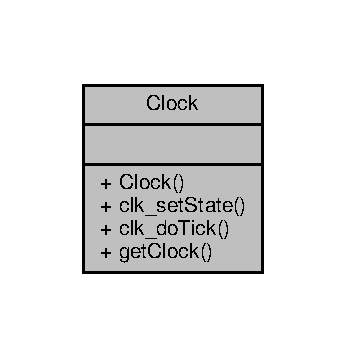
\includegraphics[width=166pt]{classClock__coll__graph}
\end{center}
\end{figure}
\subsection*{Public Member Functions}
\begin{DoxyCompactItemize}
\item 
\hyperlink{classClock_a13503a66a3130a5e3b05fc193256d955}{Clock} (int clklen)
\item 
void \hyperlink{classClock_ac941053d2f99ef4c97f7673162ced603}{clk\-\_\-set\-State} (\hyperlink{clock_8h_ade673c43995dab2f90ea5af75c33a83c}{e\-\_\-states} state)
\item 
void \hyperlink{classClock_a00feb7c247b9c897775b05ca55e21d40}{clk\-\_\-do\-Tick} ()
\item 
double \hyperlink{classClock_a4976d32d0982ac8fa5f050364ce1a701}{get\-Clock} ()
\end{DoxyCompactItemize}


\subsection{Constructor \& Destructor Documentation}
\hypertarget{classClock_a13503a66a3130a5e3b05fc193256d955}{\index{Clock@{Clock}!Clock@{Clock}}
\index{Clock@{Clock}!Clock@{Clock}}
\subsubsection[{Clock}]{\setlength{\rightskip}{0pt plus 5cm}Clock\-::\-Clock (
\begin{DoxyParamCaption}
\item[{int}]{clklen}
\end{DoxyParamCaption}
)}}\label{classClock_a13503a66a3130a5e3b05fc193256d955}


\subsection{Member Function Documentation}
\hypertarget{classClock_a00feb7c247b9c897775b05ca55e21d40}{\index{Clock@{Clock}!clk\-\_\-do\-Tick@{clk\-\_\-do\-Tick}}
\index{clk\-\_\-do\-Tick@{clk\-\_\-do\-Tick}!Clock@{Clock}}
\subsubsection[{clk\-\_\-do\-Tick}]{\setlength{\rightskip}{0pt plus 5cm}void Clock\-::clk\-\_\-do\-Tick (
\begin{DoxyParamCaption}
{}
\end{DoxyParamCaption}
)}}\label{classClock_a00feb7c247b9c897775b05ca55e21d40}
\hypertarget{classClock_ac941053d2f99ef4c97f7673162ced603}{\index{Clock@{Clock}!clk\-\_\-set\-State@{clk\-\_\-set\-State}}
\index{clk\-\_\-set\-State@{clk\-\_\-set\-State}!Clock@{Clock}}
\subsubsection[{clk\-\_\-set\-State}]{\setlength{\rightskip}{0pt plus 5cm}void Clock\-::clk\-\_\-set\-State (
\begin{DoxyParamCaption}
\item[{{\bf e\-\_\-states}}]{state}
\end{DoxyParamCaption}
)}}\label{classClock_ac941053d2f99ef4c97f7673162ced603}
\hypertarget{classClock_a4976d32d0982ac8fa5f050364ce1a701}{\index{Clock@{Clock}!get\-Clock@{get\-Clock}}
\index{get\-Clock@{get\-Clock}!Clock@{Clock}}
\subsubsection[{get\-Clock}]{\setlength{\rightskip}{0pt plus 5cm}double Clock\-::get\-Clock (
\begin{DoxyParamCaption}
{}
\end{DoxyParamCaption}
)}}\label{classClock_a4976d32d0982ac8fa5f050364ce1a701}


The documentation for this class was generated from the following files\-:\begin{DoxyCompactItemize}
\item 
\hyperlink{clock_8h}{clock.\-h}\item 
\hyperlink{clock_8cpp}{clock.\-cpp}\end{DoxyCompactItemize}

\hypertarget{classMenu}{\section{Menu Class Reference}
\label{classMenu}\index{Menu@{Menu}}
}


menu class for menu handling.  




{\ttfamily \#include $<$menu.\-h$>$}



Collaboration diagram for Menu\-:\nopagebreak
\begin{figure}[H]
\begin{center}
\leavevmode
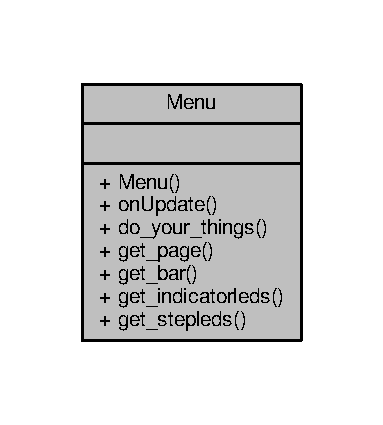
\includegraphics[width=184pt]{classMenu__coll__graph}
\end{center}
\end{figure}
\subsection*{Public Member Functions}
\begin{DoxyCompactItemize}
\item 
\hyperlink{classMenu_ad466dd83355124a6ed958430450bfe94}{Menu} ()
\item 
void \hyperlink{classMenu_af53cd78e872567d7b3261e76212bf256}{on\-Update} (void($\ast$)(int, int))
\begin{DoxyCompactList}\small\item\em on Update callback brief \end{DoxyCompactList}\item 
void \hyperlink{classMenu_aeb4138d9a42e3db932513b3880ff504c}{do\-\_\-your\-\_\-things} (int, int)
\begin{DoxyCompactList}\small\item\em this is the mainloop of menu \end{DoxyCompactList}\item 
int \hyperlink{classMenu_a4a6d32b0f1500846c567097408b7483b}{get\-\_\-page} ()
\begin{DoxyCompactList}\small\item\em returns actual page as int \end{DoxyCompactList}\item 
int \hyperlink{classMenu_ae0bb7c76d8f80158b8b793e50b0318c8}{get\-\_\-bar} ()
\begin{DoxyCompactList}\small\item\em returns actual bar position as int \end{DoxyCompactList}\item 
int \hyperlink{classMenu_aa0544dfad9c760bad1d16e6e7b31f3a7}{get\-\_\-indicatorleds} ()
\begin{DoxyCompactList}\small\item\em get indicatorleds \end{DoxyCompactList}\item 
int \hyperlink{classMenu_ae25a2b8c34b6e36f0e6fb0d05825c750}{get\-\_\-stepleds} ()
\begin{DoxyCompactList}\small\item\em get stepleds \end{DoxyCompactList}\end{DoxyCompactItemize}


\subsection{Detailed Description}
menu class for menu handling. 

It defines menu related functions and callbacks! 

\subsection{Constructor \& Destructor Documentation}
\hypertarget{classMenu_ad466dd83355124a6ed958430450bfe94}{\index{Menu@{Menu}!Menu@{Menu}}
\index{Menu@{Menu}!Menu@{Menu}}
\subsubsection[{Menu}]{\setlength{\rightskip}{0pt plus 5cm}Menu\-::\-Menu (
\begin{DoxyParamCaption}
{}
\end{DoxyParamCaption}
)}}\label{classMenu_ad466dd83355124a6ed958430450bfe94}


\subsection{Member Function Documentation}
\hypertarget{classMenu_aeb4138d9a42e3db932513b3880ff504c}{\index{Menu@{Menu}!do\-\_\-your\-\_\-things@{do\-\_\-your\-\_\-things}}
\index{do\-\_\-your\-\_\-things@{do\-\_\-your\-\_\-things}!Menu@{Menu}}
\subsubsection[{do\-\_\-your\-\_\-things}]{\setlength{\rightskip}{0pt plus 5cm}void Menu\-::do\-\_\-your\-\_\-things (
\begin{DoxyParamCaption}
\item[{int}]{fb, }
\item[{int}]{sb}
\end{DoxyParamCaption}
)}}\label{classMenu_aeb4138d9a42e3db932513b3880ff504c}


this is the mainloop of menu 

\hyperlink{classMenu}{Menu} Mainloop processes all the button and led data according to selected page needs to get updated regularly in mainloop 
\begin{DoxyParams}{Parameters}
{\em functionbuttons} & \\
\hline
{\em stepbuttons} & \\
\hline
\end{DoxyParams}
\hypertarget{classMenu_ae0bb7c76d8f80158b8b793e50b0318c8}{\index{Menu@{Menu}!get\-\_\-bar@{get\-\_\-bar}}
\index{get\-\_\-bar@{get\-\_\-bar}!Menu@{Menu}}
\subsubsection[{get\-\_\-bar}]{\setlength{\rightskip}{0pt plus 5cm}int Menu\-::get\-\_\-bar (
\begin{DoxyParamCaption}
{}
\end{DoxyParamCaption}
)}}\label{classMenu_ae0bb7c76d8f80158b8b793e50b0318c8}


returns actual bar position as int 

\hypertarget{classMenu_aa0544dfad9c760bad1d16e6e7b31f3a7}{\index{Menu@{Menu}!get\-\_\-indicatorleds@{get\-\_\-indicatorleds}}
\index{get\-\_\-indicatorleds@{get\-\_\-indicatorleds}!Menu@{Menu}}
\subsubsection[{get\-\_\-indicatorleds}]{\setlength{\rightskip}{0pt plus 5cm}int Menu\-::get\-\_\-indicatorleds (
\begin{DoxyParamCaption}
{}
\end{DoxyParamCaption}
)}}\label{classMenu_aa0544dfad9c760bad1d16e6e7b31f3a7}


get indicatorleds 

get the data for the indicator leds . process the datahandling to update the stepleds. get the according data for page. returns an int 16 states. todo\-: return 16 colors!. \hypertarget{classMenu_a4a6d32b0f1500846c567097408b7483b}{\index{Menu@{Menu}!get\-\_\-page@{get\-\_\-page}}
\index{get\-\_\-page@{get\-\_\-page}!Menu@{Menu}}
\subsubsection[{get\-\_\-page}]{\setlength{\rightskip}{0pt plus 5cm}int Menu\-::get\-\_\-page (
\begin{DoxyParamCaption}
{}
\end{DoxyParamCaption}
)}}\label{classMenu_a4a6d32b0f1500846c567097408b7483b}


returns actual page as int 

\hypertarget{classMenu_ae25a2b8c34b6e36f0e6fb0d05825c750}{\index{Menu@{Menu}!get\-\_\-stepleds@{get\-\_\-stepleds}}
\index{get\-\_\-stepleds@{get\-\_\-stepleds}!Menu@{Menu}}
\subsubsection[{get\-\_\-stepleds}]{\setlength{\rightskip}{0pt plus 5cm}int Menu\-::get\-\_\-stepleds (
\begin{DoxyParamCaption}
{}
\end{DoxyParamCaption}
)}}\label{classMenu_ae25a2b8c34b6e36f0e6fb0d05825c750}


get stepleds 

process the datahandling to update the stepleds. get the according data for page. returns an int 16 states. todo\-: return 16 colors!. \hypertarget{classMenu_af53cd78e872567d7b3261e76212bf256}{\index{Menu@{Menu}!on\-Update@{on\-Update}}
\index{on\-Update@{on\-Update}!Menu@{Menu}}
\subsubsection[{on\-Update}]{\setlength{\rightskip}{0pt plus 5cm}void Menu\-::on\-Update (
\begin{DoxyParamCaption}
\item[{void($\ast$)(int, int)}]{function}
\end{DoxyParamCaption}
)}}\label{classMenu_af53cd78e872567d7b3261e76212bf256}


on Update callback brief 

on\-Update callback detail 
\begin{DoxyParams}{Parameters}
{\em function} & to call. gets called by ??. and processes the events \\
\hline
\end{DoxyParams}


The documentation for this class was generated from the following files\-:\begin{DoxyCompactItemize}
\item 
\hyperlink{menu_8h}{menu.\-h}\item 
\hyperlink{menu_8cpp}{menu.\-cpp}\end{DoxyCompactItemize}

\hypertarget{classSequence}{\section{Sequence Class Reference}
\label{classSequence}\index{Sequence@{Sequence}}
}


\hyperlink{classSequence}{Sequence} class.  




{\ttfamily \#include $<$sequence.\-h$>$}



Collaboration diagram for Sequence\-:\nopagebreak
\begin{figure}[H]
\begin{center}
\leavevmode
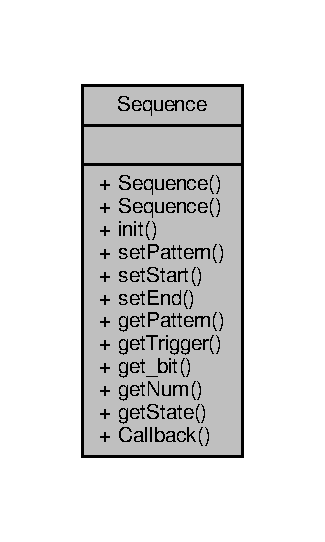
\includegraphics[width=156pt]{classSequence__coll__graph}
\end{center}
\end{figure}
\subsection*{Public Member Functions}
\begin{DoxyCompactItemize}
\item 
\hyperlink{classSequence_a532b7e8df6ff6b2f990c14ae97859ca2}{Sequence} ()
\item 
\hyperlink{classSequence_aa46c51af61f19f47edbcb6865ec2eb21}{Sequence} (int trknum)
\item 
void \hyperlink{classSequence_a3866247a6a89a872514c3261b44c7e84}{init} (int)
\item 
void \hyperlink{classSequence_a4e4fe35ef98f961f64b6ff0fb0a6070b}{set\-Pattern} (int pattern)
\item 
void \hyperlink{classSequence_a63497de29b000ab800a9bfd862098010}{set\-Start} (int start)
\item 
void \hyperlink{classSequence_acd5fae49c72278d6d60ebb636f00a1b0}{set\-End} (int end)
\item 
int \hyperlink{classSequence_a0be7ca1c73194895111720e925e5f81c}{get\-Pattern} ()
\item 
bool \hyperlink{classSequence_ab400118246dd9437e1b4ea256bbdb626}{get\-Trigger} (int position)
\item 
bool \hyperlink{classSequence_a0aa238e326a703b831cf7dc5d873342b}{get\-\_\-bit} (int val, int pos)
\item 
int \hyperlink{classSequence_a5d749697a9eace5524ace54f323356bb}{get\-Num} ()
\item 
\hyperlink{namespaceSequenceEnum_ac7ea8369c971b81acfe5a1d63a10ebe3}{Sequence\-Enum\-::e\-\_\-run\-States} \hyperlink{classSequence_a45c5eaacd6489bc001ff5fd8d8dc8ff9}{get\-State} ()
\end{DoxyCompactItemize}
\subsection*{Static Public Member Functions}
\begin{DoxyCompactItemize}
\item 
static void \hyperlink{classSequence_ab155aaa37dda5a6e916afeb68a7e8edf}{Callback} (\hyperlink{classSequence}{Sequence} $\ast$instance, int x)
\end{DoxyCompactItemize}


\subsection{Detailed Description}
\hyperlink{classSequence}{Sequence} class. 

This is the \hyperlink{classSequence}{Sequence} class.\par
 it defines one sequence of the pattern! 

\subsection{Constructor \& Destructor Documentation}
\hypertarget{classSequence_a532b7e8df6ff6b2f990c14ae97859ca2}{\index{Sequence@{Sequence}!Sequence@{Sequence}}
\index{Sequence@{Sequence}!Sequence@{Sequence}}
\subsubsection[{Sequence}]{\setlength{\rightskip}{0pt plus 5cm}Sequence\-::\-Sequence (
\begin{DoxyParamCaption}
{}
\end{DoxyParamCaption}
)}}\label{classSequence_a532b7e8df6ff6b2f990c14ae97859ca2}
\hypertarget{classSequence_aa46c51af61f19f47edbcb6865ec2eb21}{\index{Sequence@{Sequence}!Sequence@{Sequence}}
\index{Sequence@{Sequence}!Sequence@{Sequence}}
\subsubsection[{Sequence}]{\setlength{\rightskip}{0pt plus 5cm}Sequence\-::\-Sequence (
\begin{DoxyParamCaption}
\item[{int}]{trknum}
\end{DoxyParamCaption}
)}}\label{classSequence_aa46c51af61f19f47edbcb6865ec2eb21}


\subsection{Member Function Documentation}
\hypertarget{classSequence_ab155aaa37dda5a6e916afeb68a7e8edf}{\index{Sequence@{Sequence}!Callback@{Callback}}
\index{Callback@{Callback}!Sequence@{Sequence}}
\subsubsection[{Callback}]{\setlength{\rightskip}{0pt plus 5cm}static void Sequence\-::\-Callback (
\begin{DoxyParamCaption}
\item[{{\bf Sequence} $\ast$}]{instance, }
\item[{int}]{x}
\end{DoxyParamCaption}
)\hspace{0.3cm}{\ttfamily [static]}}}\label{classSequence_ab155aaa37dda5a6e916afeb68a7e8edf}
\hypertarget{classSequence_a0aa238e326a703b831cf7dc5d873342b}{\index{Sequence@{Sequence}!get\-\_\-bit@{get\-\_\-bit}}
\index{get\-\_\-bit@{get\-\_\-bit}!Sequence@{Sequence}}
\subsubsection[{get\-\_\-bit}]{\setlength{\rightskip}{0pt plus 5cm}bool Sequence\-::get\-\_\-bit (
\begin{DoxyParamCaption}
\item[{int}]{val, }
\item[{int}]{pos}
\end{DoxyParamCaption}
)}}\label{classSequence_a0aa238e326a703b831cf7dc5d873342b}
\hypertarget{classSequence_a5d749697a9eace5524ace54f323356bb}{\index{Sequence@{Sequence}!get\-Num@{get\-Num}}
\index{get\-Num@{get\-Num}!Sequence@{Sequence}}
\subsubsection[{get\-Num}]{\setlength{\rightskip}{0pt plus 5cm}int Sequence\-::get\-Num (
\begin{DoxyParamCaption}
{}
\end{DoxyParamCaption}
)}}\label{classSequence_a5d749697a9eace5524ace54f323356bb}
\hypertarget{classSequence_a0be7ca1c73194895111720e925e5f81c}{\index{Sequence@{Sequence}!get\-Pattern@{get\-Pattern}}
\index{get\-Pattern@{get\-Pattern}!Sequence@{Sequence}}
\subsubsection[{get\-Pattern}]{\setlength{\rightskip}{0pt plus 5cm}int Sequence\-::get\-Pattern (
\begin{DoxyParamCaption}
{}
\end{DoxyParamCaption}
)}}\label{classSequence_a0be7ca1c73194895111720e925e5f81c}
\hypertarget{classSequence_a45c5eaacd6489bc001ff5fd8d8dc8ff9}{\index{Sequence@{Sequence}!get\-State@{get\-State}}
\index{get\-State@{get\-State}!Sequence@{Sequence}}
\subsubsection[{get\-State}]{\setlength{\rightskip}{0pt plus 5cm}{\bf Sequence\-Enum\-::e\-\_\-run\-States} Sequence\-::get\-State (
\begin{DoxyParamCaption}
{}
\end{DoxyParamCaption}
)}}\label{classSequence_a45c5eaacd6489bc001ff5fd8d8dc8ff9}
\hypertarget{classSequence_ab400118246dd9437e1b4ea256bbdb626}{\index{Sequence@{Sequence}!get\-Trigger@{get\-Trigger}}
\index{get\-Trigger@{get\-Trigger}!Sequence@{Sequence}}
\subsubsection[{get\-Trigger}]{\setlength{\rightskip}{0pt plus 5cm}bool Sequence\-::get\-Trigger (
\begin{DoxyParamCaption}
\item[{int}]{position}
\end{DoxyParamCaption}
)}}\label{classSequence_ab400118246dd9437e1b4ea256bbdb626}
\hypertarget{classSequence_a3866247a6a89a872514c3261b44c7e84}{\index{Sequence@{Sequence}!init@{init}}
\index{init@{init}!Sequence@{Sequence}}
\subsubsection[{init}]{\setlength{\rightskip}{0pt plus 5cm}void Sequence\-::init (
\begin{DoxyParamCaption}
\item[{int}]{trknum}
\end{DoxyParamCaption}
)}}\label{classSequence_a3866247a6a89a872514c3261b44c7e84}
\hypertarget{classSequence_acd5fae49c72278d6d60ebb636f00a1b0}{\index{Sequence@{Sequence}!set\-End@{set\-End}}
\index{set\-End@{set\-End}!Sequence@{Sequence}}
\subsubsection[{set\-End}]{\setlength{\rightskip}{0pt plus 5cm}void Sequence\-::set\-End (
\begin{DoxyParamCaption}
\item[{int}]{end}
\end{DoxyParamCaption}
)}}\label{classSequence_acd5fae49c72278d6d60ebb636f00a1b0}
\hypertarget{classSequence_a4e4fe35ef98f961f64b6ff0fb0a6070b}{\index{Sequence@{Sequence}!set\-Pattern@{set\-Pattern}}
\index{set\-Pattern@{set\-Pattern}!Sequence@{Sequence}}
\subsubsection[{set\-Pattern}]{\setlength{\rightskip}{0pt plus 5cm}void Sequence\-::set\-Pattern (
\begin{DoxyParamCaption}
\item[{int}]{pattern}
\end{DoxyParamCaption}
)}}\label{classSequence_a4e4fe35ef98f961f64b6ff0fb0a6070b}
\hypertarget{classSequence_a63497de29b000ab800a9bfd862098010}{\index{Sequence@{Sequence}!set\-Start@{set\-Start}}
\index{set\-Start@{set\-Start}!Sequence@{Sequence}}
\subsubsection[{set\-Start}]{\setlength{\rightskip}{0pt plus 5cm}void Sequence\-::set\-Start (
\begin{DoxyParamCaption}
\item[{int}]{start}
\end{DoxyParamCaption}
)}}\label{classSequence_a63497de29b000ab800a9bfd862098010}


The documentation for this class was generated from the following files\-:\begin{DoxyCompactItemize}
\item 
\hyperlink{sequence_8h}{sequence.\-h}\item 
\hyperlink{sequence_8cpp}{sequence.\-cpp}\end{DoxyCompactItemize}

\hypertarget{structSequenceEnum_1_1SequenceMeta}{\section{Sequence\-Enum\-:\-:Sequence\-Meta Struct Reference}
\label{structSequenceEnum_1_1SequenceMeta}\index{Sequence\-Enum\-::\-Sequence\-Meta@{Sequence\-Enum\-::\-Sequence\-Meta}}
}


some ssquence metadata for internal handling  




{\ttfamily \#include $<$sequence.\-h$>$}



Collaboration diagram for Sequence\-Enum\-:\-:Sequence\-Meta\-:\nopagebreak
\begin{figure}[H]
\begin{center}
\leavevmode
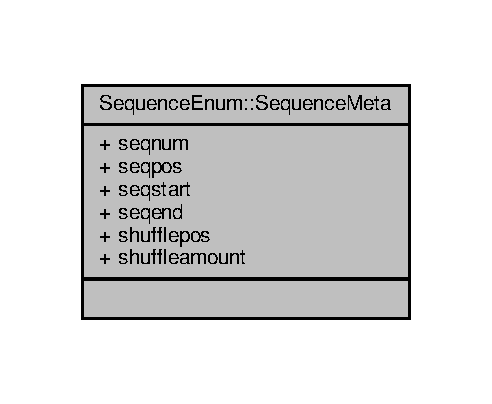
\includegraphics[width=236pt]{structSequenceEnum_1_1SequenceMeta__coll__graph}
\end{center}
\end{figure}
\subsection*{Public Attributes}
\begin{DoxyCompactItemize}
\item 
int \hyperlink{structSequenceEnum_1_1SequenceMeta_aeaa7178f934040cf56cde8520d50d5ae}{seqnum}
\item 
int \hyperlink{structSequenceEnum_1_1SequenceMeta_a4592f8f35b0dc3633cf0b8d233ad9b6e}{seqpos}
\item 
int \hyperlink{structSequenceEnum_1_1SequenceMeta_af53e20202a4cb12d68c8d872144503c2}{seqstart}
\begin{DoxyCompactList}\small\item\em Position of play pointer in sequence. \end{DoxyCompactList}\item 
int \hyperlink{structSequenceEnum_1_1SequenceMeta_a1cf3e614f05a79a98016ef829c50b958}{seqend}
\begin{DoxyCompactList}\small\item\em start position for play pointer \end{DoxyCompactList}\item 
int \hyperlink{structSequenceEnum_1_1SequenceMeta_ac76334a90ea5cdcefa31a099a35fa4dc}{shufflepos}
\begin{DoxyCompactList}\small\item\em end for play pointer \end{DoxyCompactList}\item 
int \hyperlink{structSequenceEnum_1_1SequenceMeta_a368101eef07df62d77a16bd2715f7d19}{shuffleamount}
\begin{DoxyCompactList}\small\item\em position to shuffle \end{DoxyCompactList}\end{DoxyCompactItemize}


\subsection{Detailed Description}
some ssquence metadata for internal handling 

\subsection{Member Data Documentation}
\hypertarget{structSequenceEnum_1_1SequenceMeta_a1cf3e614f05a79a98016ef829c50b958}{\index{Sequence\-Enum\-::\-Sequence\-Meta@{Sequence\-Enum\-::\-Sequence\-Meta}!seqend@{seqend}}
\index{seqend@{seqend}!SequenceEnum::SequenceMeta@{Sequence\-Enum\-::\-Sequence\-Meta}}
\subsubsection[{seqend}]{\setlength{\rightskip}{0pt plus 5cm}int Sequence\-Enum\-::\-Sequence\-Meta\-::seqend}}\label{structSequenceEnum_1_1SequenceMeta_a1cf3e614f05a79a98016ef829c50b958}


start position for play pointer 

\hypertarget{structSequenceEnum_1_1SequenceMeta_aeaa7178f934040cf56cde8520d50d5ae}{\index{Sequence\-Enum\-::\-Sequence\-Meta@{Sequence\-Enum\-::\-Sequence\-Meta}!seqnum@{seqnum}}
\index{seqnum@{seqnum}!SequenceEnum::SequenceMeta@{Sequence\-Enum\-::\-Sequence\-Meta}}
\subsubsection[{seqnum}]{\setlength{\rightskip}{0pt plus 5cm}int Sequence\-Enum\-::\-Sequence\-Meta\-::seqnum}}\label{structSequenceEnum_1_1SequenceMeta_aeaa7178f934040cf56cde8520d50d5ae}
Internal sequence Number \hypertarget{structSequenceEnum_1_1SequenceMeta_a4592f8f35b0dc3633cf0b8d233ad9b6e}{\index{Sequence\-Enum\-::\-Sequence\-Meta@{Sequence\-Enum\-::\-Sequence\-Meta}!seqpos@{seqpos}}
\index{seqpos@{seqpos}!SequenceEnum::SequenceMeta@{Sequence\-Enum\-::\-Sequence\-Meta}}
\subsubsection[{seqpos}]{\setlength{\rightskip}{0pt plus 5cm}int Sequence\-Enum\-::\-Sequence\-Meta\-::seqpos}}\label{structSequenceEnum_1_1SequenceMeta_a4592f8f35b0dc3633cf0b8d233ad9b6e}
\hypertarget{structSequenceEnum_1_1SequenceMeta_af53e20202a4cb12d68c8d872144503c2}{\index{Sequence\-Enum\-::\-Sequence\-Meta@{Sequence\-Enum\-::\-Sequence\-Meta}!seqstart@{seqstart}}
\index{seqstart@{seqstart}!SequenceEnum::SequenceMeta@{Sequence\-Enum\-::\-Sequence\-Meta}}
\subsubsection[{seqstart}]{\setlength{\rightskip}{0pt plus 5cm}int Sequence\-Enum\-::\-Sequence\-Meta\-::seqstart}}\label{structSequenceEnum_1_1SequenceMeta_af53e20202a4cb12d68c8d872144503c2}


Position of play pointer in sequence. 

\hypertarget{structSequenceEnum_1_1SequenceMeta_a368101eef07df62d77a16bd2715f7d19}{\index{Sequence\-Enum\-::\-Sequence\-Meta@{Sequence\-Enum\-::\-Sequence\-Meta}!shuffleamount@{shuffleamount}}
\index{shuffleamount@{shuffleamount}!SequenceEnum::SequenceMeta@{Sequence\-Enum\-::\-Sequence\-Meta}}
\subsubsection[{shuffleamount}]{\setlength{\rightskip}{0pt plus 5cm}int Sequence\-Enum\-::\-Sequence\-Meta\-::shuffleamount}}\label{structSequenceEnum_1_1SequenceMeta_a368101eef07df62d77a16bd2715f7d19}


position to shuffle 

\hypertarget{structSequenceEnum_1_1SequenceMeta_ac76334a90ea5cdcefa31a099a35fa4dc}{\index{Sequence\-Enum\-::\-Sequence\-Meta@{Sequence\-Enum\-::\-Sequence\-Meta}!shufflepos@{shufflepos}}
\index{shufflepos@{shufflepos}!SequenceEnum::SequenceMeta@{Sequence\-Enum\-::\-Sequence\-Meta}}
\subsubsection[{shufflepos}]{\setlength{\rightskip}{0pt plus 5cm}int Sequence\-Enum\-::\-Sequence\-Meta\-::shufflepos}}\label{structSequenceEnum_1_1SequenceMeta_ac76334a90ea5cdcefa31a099a35fa4dc}


end for play pointer 



The documentation for this struct was generated from the following file\-:\begin{DoxyCompactItemize}
\item 
\hyperlink{sequence_8h}{sequence.\-h}\end{DoxyCompactItemize}

\hypertarget{structSequenceEnum_1_1StepData}{\section{Sequence\-Enum\-:\-:Step\-Data Struct Reference}
\label{structSequenceEnum_1_1StepData}\index{Sequence\-Enum\-::\-Step\-Data@{Sequence\-Enum\-::\-Step\-Data}}
}


Basic struct of one step -\/ data. used on all step data operations.  




{\ttfamily \#include $<$sequence.\-h$>$}



Collaboration diagram for Sequence\-Enum\-:\-:Step\-Data\-:\nopagebreak
\begin{figure}[H]
\begin{center}
\leavevmode
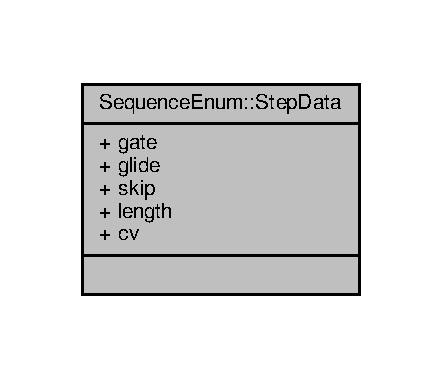
\includegraphics[width=212pt]{structSequenceEnum_1_1StepData__coll__graph}
\end{center}
\end{figure}
\subsection*{Public Attributes}
\begin{DoxyCompactItemize}
\item 
bool \hyperlink{structSequenceEnum_1_1StepData_a597603a9b2d9eaf490f659dfcbbee804}{gate}
\item 
bool \hyperlink{structSequenceEnum_1_1StepData_a067c43b25989443622354b94ddee2799}{glide}
\item 
bool \hyperlink{structSequenceEnum_1_1StepData_ac3146c1d3252ee1326959fa3b8191490}{skip}
\item 
bool \hyperlink{structSequenceEnum_1_1StepData_a493978b8534c96c86e10b51be7f4bf62}{length} \mbox{[}4\mbox{]}
\item 
int \hyperlink{structSequenceEnum_1_1StepData_a94070c904112e9bbc18ac7e63ea1d8d0}{cv}
\end{DoxyCompactItemize}


\subsection{Detailed Description}
Basic struct of one step -\/ data. used on all step data operations. 

\subsection{Member Data Documentation}
\hypertarget{structSequenceEnum_1_1StepData_a94070c904112e9bbc18ac7e63ea1d8d0}{\index{Sequence\-Enum\-::\-Step\-Data@{Sequence\-Enum\-::\-Step\-Data}!cv@{cv}}
\index{cv@{cv}!SequenceEnum::StepData@{Sequence\-Enum\-::\-Step\-Data}}
\subsubsection[{cv}]{\setlength{\rightskip}{0pt plus 5cm}int Sequence\-Enum\-::\-Step\-Data\-::cv}}\label{structSequenceEnum_1_1StepData_a94070c904112e9bbc18ac7e63ea1d8d0}
Cv Value 4 step \hypertarget{structSequenceEnum_1_1StepData_a597603a9b2d9eaf490f659dfcbbee804}{\index{Sequence\-Enum\-::\-Step\-Data@{Sequence\-Enum\-::\-Step\-Data}!gate@{gate}}
\index{gate@{gate}!SequenceEnum::StepData@{Sequence\-Enum\-::\-Step\-Data}}
\subsubsection[{gate}]{\setlength{\rightskip}{0pt plus 5cm}bool Sequence\-Enum\-::\-Step\-Data\-::gate}}\label{structSequenceEnum_1_1StepData_a597603a9b2d9eaf490f659dfcbbee804}
Gate O\-N ! \hypertarget{structSequenceEnum_1_1StepData_a067c43b25989443622354b94ddee2799}{\index{Sequence\-Enum\-::\-Step\-Data@{Sequence\-Enum\-::\-Step\-Data}!glide@{glide}}
\index{glide@{glide}!SequenceEnum::StepData@{Sequence\-Enum\-::\-Step\-Data}}
\subsubsection[{glide}]{\setlength{\rightskip}{0pt plus 5cm}bool Sequence\-Enum\-::\-Step\-Data\-::glide}}\label{structSequenceEnum_1_1StepData_a067c43b25989443622354b94ddee2799}
Glide this? \hypertarget{structSequenceEnum_1_1StepData_a493978b8534c96c86e10b51be7f4bf62}{\index{Sequence\-Enum\-::\-Step\-Data@{Sequence\-Enum\-::\-Step\-Data}!length@{length}}
\index{length@{length}!SequenceEnum::StepData@{Sequence\-Enum\-::\-Step\-Data}}
\subsubsection[{length}]{\setlength{\rightskip}{0pt plus 5cm}bool Sequence\-Enum\-::\-Step\-Data\-::length\mbox{[}4\mbox{]}}}\label{structSequenceEnum_1_1StepData_a493978b8534c96c86e10b51be7f4bf62}
Gate length \hypertarget{structSequenceEnum_1_1StepData_ac3146c1d3252ee1326959fa3b8191490}{\index{Sequence\-Enum\-::\-Step\-Data@{Sequence\-Enum\-::\-Step\-Data}!skip@{skip}}
\index{skip@{skip}!SequenceEnum::StepData@{Sequence\-Enum\-::\-Step\-Data}}
\subsubsection[{skip}]{\setlength{\rightskip}{0pt plus 5cm}bool Sequence\-Enum\-::\-Step\-Data\-::skip}}\label{structSequenceEnum_1_1StepData_ac3146c1d3252ee1326959fa3b8191490}
Skip ? 

The documentation for this struct was generated from the following file\-:\begin{DoxyCompactItemize}
\item 
\hyperlink{sequence_8h}{sequence.\-h}\end{DoxyCompactItemize}

\chapter{File Documentation}
\hypertarget{_8ino_8cpp}{\section{.ino.\-cpp File Reference}
\label{_8ino_8cpp}\index{.\-ino.\-cpp@{.\-ino.\-cpp}}
}
{\ttfamily \#include \char`\"{}Arduino.\-h\char`\"{}}\\*
{\ttfamily \#include $<$Due\-Timer.\-h$>$}\\*
{\ttfamily \#include $<$U\-A\-R\-T\-Class.\-h$>$}\\*
{\ttfamily \#include $<$variant.\-h$>$}\\*
{\ttfamily \#include $<$wiring.\-h$>$}\\*
{\ttfamily \#include $<$wiring\-\_\-constants.\-h$>$}\\*
{\ttfamily \#include \char`\"{}debug.\-h\char`\"{}}\\*
{\ttfamily \#include \char`\"{}globals.\-h\char`\"{}}\\*
{\ttfamily \#include \char`\"{}menu.\-h\char`\"{}}\\*
{\ttfamily \#include \char`\"{}porthardware.\-h\char`\"{}}\\*
{\ttfamily \#include \char`\"{}sequence.\-h\char`\"{}}\\*
{\ttfamily \#include \char`\"{}ledquencer.\-ino\char`\"{}}\\*
Include dependency graph for .ino.\-cpp\-:
\nopagebreak
\begin{figure}[H]
\begin{center}
\leavevmode
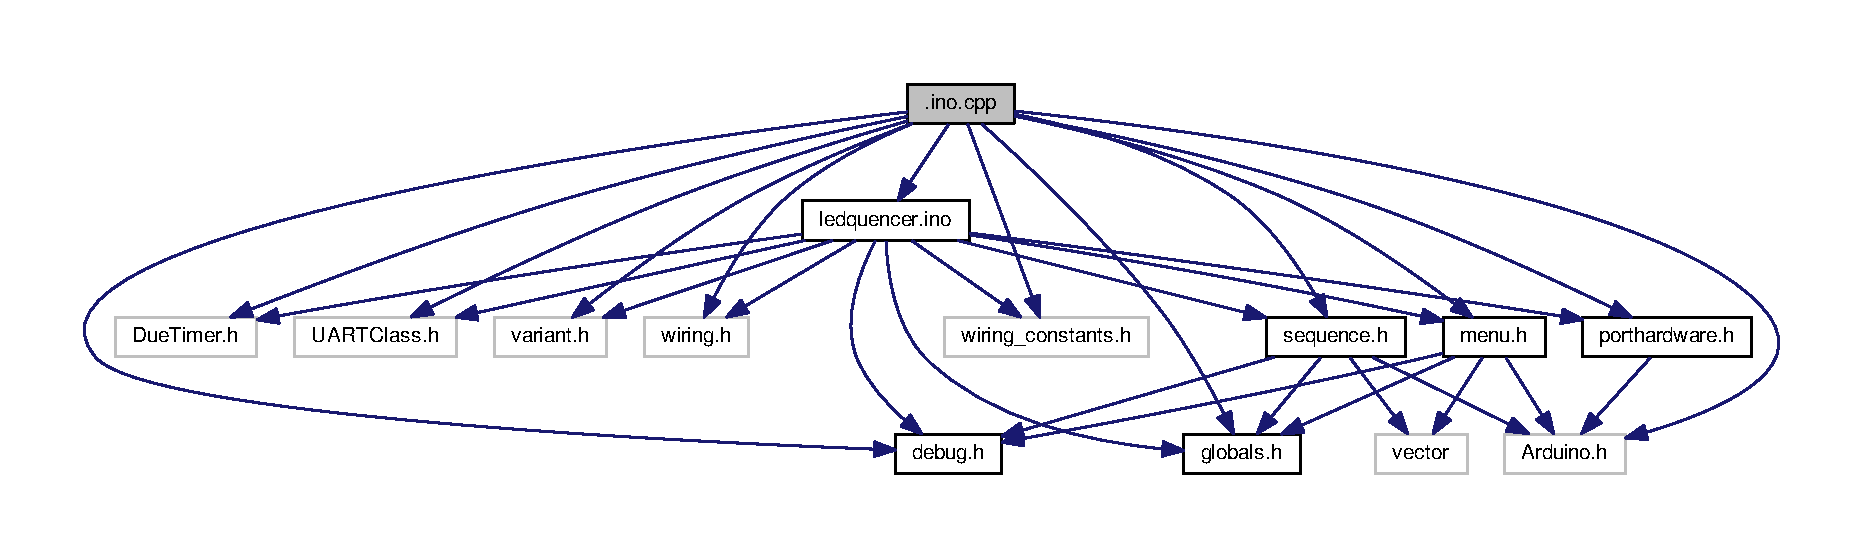
\includegraphics[width=350pt]{_8ino_8cpp__incl}
\end{center}
\end{figure}
\subsection*{Functions}
\begin{DoxyCompactItemize}
\item 
void \hyperlink{_8ino_8cpp_a859467c5035bc8e63b57dfe199caec30}{test} (int page, int buttons)
\item 
void \hyperlink{_8ino_8cpp_a4fc01d736fe50cf5b977f755b675f11d}{setup} ()
\item 
void \hyperlink{_8ino_8cpp_afe461d27b9c48d5921c00d521181f12f}{loop} ()
\item 
void \hyperlink{_8ino_8cpp_a36f33b2b623ea070c4ebccc7464ef489}{timer0\-\_\-handler} ()
\item 
void \hyperlink{_8ino_8cpp_a859aab5acbfa52240ec73ba136fb6bf3}{timer1\-\_\-handler} ()
\item 
void \hyperlink{_8ino_8cpp_a7cbb97684327369274bcf81b967c3a6b}{timer2\-\_\-handler} ()
\item 
void \hyperlink{_8ino_8cpp_a21338471d58456b6ec2c6b0070e44d67}{timer3\-\_\-handler} ()
\item 
void \hyperlink{_8ino_8cpp_a92c00e5adb1836741614c6492982e306}{alive1} ()
\end{DoxyCompactItemize}


\subsection{Function Documentation}
\hypertarget{_8ino_8cpp_a92c00e5adb1836741614c6492982e306}{\index{.\-ino.\-cpp@{.\-ino.\-cpp}!alive1@{alive1}}
\index{alive1@{alive1}!.ino.cpp@{.\-ino.\-cpp}}
\subsubsection[{alive1}]{\setlength{\rightskip}{0pt plus 5cm}void alive1 (
\begin{DoxyParamCaption}
{}
\end{DoxyParamCaption}
)}}\label{_8ino_8cpp_a92c00e5adb1836741614c6492982e306}
\hypertarget{_8ino_8cpp_afe461d27b9c48d5921c00d521181f12f}{\index{.\-ino.\-cpp@{.\-ino.\-cpp}!loop@{loop}}
\index{loop@{loop}!.ino.cpp@{.\-ino.\-cpp}}
\subsubsection[{loop}]{\setlength{\rightskip}{0pt plus 5cm}void loop (
\begin{DoxyParamCaption}
{}
\end{DoxyParamCaption}
)}}\label{_8ino_8cpp_afe461d27b9c48d5921c00d521181f12f}
\hypertarget{_8ino_8cpp_a4fc01d736fe50cf5b977f755b675f11d}{\index{.\-ino.\-cpp@{.\-ino.\-cpp}!setup@{setup}}
\index{setup@{setup}!.ino.cpp@{.\-ino.\-cpp}}
\subsubsection[{setup}]{\setlength{\rightskip}{0pt plus 5cm}void setup (
\begin{DoxyParamCaption}
{}
\end{DoxyParamCaption}
)}}\label{_8ino_8cpp_a4fc01d736fe50cf5b977f755b675f11d}
\hypertarget{_8ino_8cpp_a859467c5035bc8e63b57dfe199caec30}{\index{.\-ino.\-cpp@{.\-ino.\-cpp}!test@{test}}
\index{test@{test}!.ino.cpp@{.\-ino.\-cpp}}
\subsubsection[{test}]{\setlength{\rightskip}{0pt plus 5cm}void test (
\begin{DoxyParamCaption}
\item[{int}]{page, }
\item[{int}]{buttons}
\end{DoxyParamCaption}
)}}\label{_8ino_8cpp_a859467c5035bc8e63b57dfe199caec30}
\hypertarget{_8ino_8cpp_a36f33b2b623ea070c4ebccc7464ef489}{\index{.\-ino.\-cpp@{.\-ino.\-cpp}!timer0\-\_\-handler@{timer0\-\_\-handler}}
\index{timer0\-\_\-handler@{timer0\-\_\-handler}!.ino.cpp@{.\-ino.\-cpp}}
\subsubsection[{timer0\-\_\-handler}]{\setlength{\rightskip}{0pt plus 5cm}void timer0\-\_\-handler (
\begin{DoxyParamCaption}
{}
\end{DoxyParamCaption}
)}}\label{_8ino_8cpp_a36f33b2b623ea070c4ebccc7464ef489}
\hypertarget{_8ino_8cpp_a859aab5acbfa52240ec73ba136fb6bf3}{\index{.\-ino.\-cpp@{.\-ino.\-cpp}!timer1\-\_\-handler@{timer1\-\_\-handler}}
\index{timer1\-\_\-handler@{timer1\-\_\-handler}!.ino.cpp@{.\-ino.\-cpp}}
\subsubsection[{timer1\-\_\-handler}]{\setlength{\rightskip}{0pt plus 5cm}void timer1\-\_\-handler (
\begin{DoxyParamCaption}
{}
\end{DoxyParamCaption}
)}}\label{_8ino_8cpp_a859aab5acbfa52240ec73ba136fb6bf3}
\hypertarget{_8ino_8cpp_a7cbb97684327369274bcf81b967c3a6b}{\index{.\-ino.\-cpp@{.\-ino.\-cpp}!timer2\-\_\-handler@{timer2\-\_\-handler}}
\index{timer2\-\_\-handler@{timer2\-\_\-handler}!.ino.cpp@{.\-ino.\-cpp}}
\subsubsection[{timer2\-\_\-handler}]{\setlength{\rightskip}{0pt plus 5cm}void timer2\-\_\-handler (
\begin{DoxyParamCaption}
{}
\end{DoxyParamCaption}
)}}\label{_8ino_8cpp_a7cbb97684327369274bcf81b967c3a6b}
\hypertarget{_8ino_8cpp_a21338471d58456b6ec2c6b0070e44d67}{\index{.\-ino.\-cpp@{.\-ino.\-cpp}!timer3\-\_\-handler@{timer3\-\_\-handler}}
\index{timer3\-\_\-handler@{timer3\-\_\-handler}!.ino.cpp@{.\-ino.\-cpp}}
\subsubsection[{timer3\-\_\-handler}]{\setlength{\rightskip}{0pt plus 5cm}void timer3\-\_\-handler (
\begin{DoxyParamCaption}
{}
\end{DoxyParamCaption}
)}}\label{_8ino_8cpp_a21338471d58456b6ec2c6b0070e44d67}

\hypertarget{bushardware_8h}{\section{bushardware.\-h File Reference}
\label{bushardware_8h}\index{bushardware.\-h@{bushardware.\-h}}
}
{\ttfamily \#include $<$Fast\-L\-E\-D.\-h$>$}\\*
{\ttfamily \#include $<$pixeltypes.\-h$>$}\\*
{\ttfamily \#include $<$sam3xa/include/instance/instance\-\_\-pioa.\-h$>$}\\*
{\ttfamily \#include $<$U\-A\-R\-T\-Class.\-h$>$}\\*
{\ttfamily \#include $<$variant.\-h$>$}\\*
{\ttfamily \#include $<$Wire.\-h$>$}\\*
{\ttfamily \#include \char`\"{}Adafruit\-\_\-\-M\-P\-R121.\-h\char`\"{}}\\*
{\ttfamily \#include $<$Adafruit\-\_\-\-Neo\-Pixel.\-h$>$}\\*
Include dependency graph for bushardware.\-h\-:\nopagebreak
\begin{figure}[H]
\begin{center}
\leavevmode
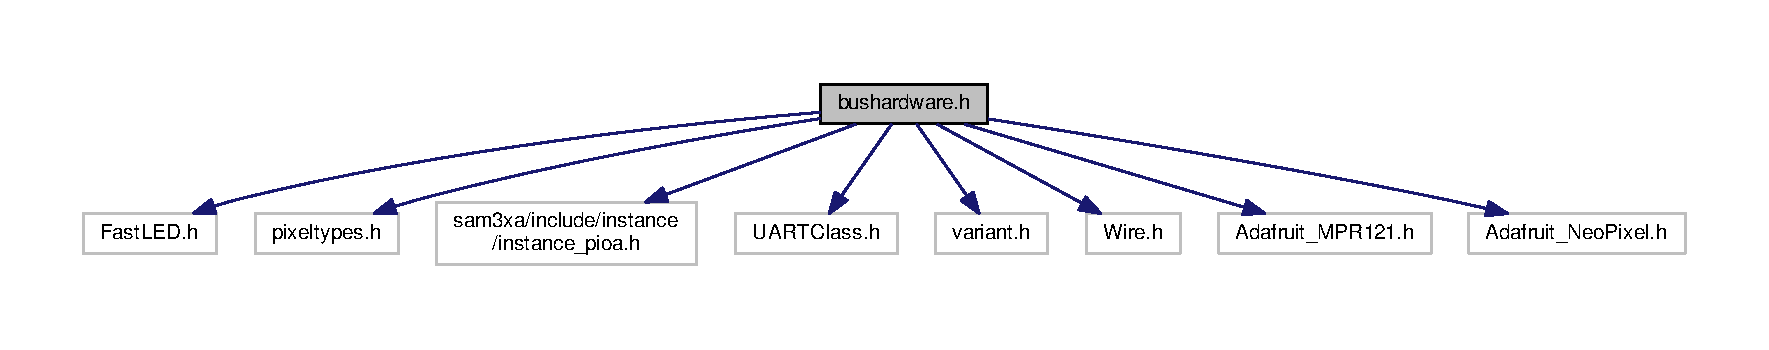
\includegraphics[width=350pt]{bushardware_8h__incl}
\end{center}
\end{figure}
\subsection*{Macros}
\begin{DoxyCompactItemize}
\item 
\#define \hyperlink{bushardware_8h_adad67fe595ea440c8f8247ec2cddf070}{D\-A\-T\-A\-\_\-\-P\-I\-N}~6
\item 
\#define \hyperlink{bushardware_8h_a4c4ae9a4146ce8d6a5debc90300d9abd}{N\-U\-M\-\_\-\-L\-E\-D\-S}~40
\end{DoxyCompactItemize}
\subsection*{Functions}
\begin{DoxyCompactItemize}
\item 
void \hyperlink{bushardware_8h_a5fa2c6d71783408acbdfa7046ecc777f}{show\-Leds} ()
\item 
void \hyperlink{bushardware_8h_adf3d0f6e1a9dd64fb3ec03ec0e662bfe}{read\-Buttons} ()
\item 
void \hyperlink{bushardware_8h_a7b55b33f80d664f78718fdb04b0b9f7c}{set\-Debounce} ()
\item 
void \hyperlink{bushardware_8h_ad8d6aca3d85765fb35287d8f9bad21d1}{portsetup} ()
\end{DoxyCompactItemize}
\subsection*{Variables}
\begin{DoxyCompactItemize}
\item 
C\-R\-G\-B \hyperlink{bushardware_8h_a1b4f26a01e11d7eb2848bc41b0f6dd9d}{leds} \mbox{[}\hyperlink{bushardware_8h_a4c4ae9a4146ce8d6a5debc90300d9abd}{N\-U\-M\-\_\-\-L\-E\-D\-S}\mbox{]}
\item 
Adafruit\-\_\-\-M\-P\-R121 \hyperlink{bushardware_8h_a5fde9cee1f1e57f9ee8d7203e9001669}{touchboard} \mbox{[}4\mbox{]} = \{ Adafruit\-\_\-\-M\-P\-R121() \}
\item 
Adafruit\-\_\-\-Neo\-Pixel \hyperlink{bushardware_8h_acf2771bd8bfaf855bbcc6c30301bf380}{strip} = Adafruit\-\_\-\-Neo\-Pixel(40, \hyperlink{bushardware_8h_adad67fe595ea440c8f8247ec2cddf070}{D\-A\-T\-A\-\_\-\-P\-I\-N}, N\-E\-O\-\_\-\-G\-R\-B + N\-E\-O\-\_\-\-K\-H\-Z800)
\end{DoxyCompactItemize}


\subsection{Macro Definition Documentation}
\hypertarget{bushardware_8h_adad67fe595ea440c8f8247ec2cddf070}{\index{bushardware.\-h@{bushardware.\-h}!D\-A\-T\-A\-\_\-\-P\-I\-N@{D\-A\-T\-A\-\_\-\-P\-I\-N}}
\index{D\-A\-T\-A\-\_\-\-P\-I\-N@{D\-A\-T\-A\-\_\-\-P\-I\-N}!bushardware.h@{bushardware.\-h}}
\subsubsection[{D\-A\-T\-A\-\_\-\-P\-I\-N}]{\setlength{\rightskip}{0pt plus 5cm}\#define D\-A\-T\-A\-\_\-\-P\-I\-N~6}}\label{bushardware_8h_adad67fe595ea440c8f8247ec2cddf070}
\hypertarget{bushardware_8h_a4c4ae9a4146ce8d6a5debc90300d9abd}{\index{bushardware.\-h@{bushardware.\-h}!N\-U\-M\-\_\-\-L\-E\-D\-S@{N\-U\-M\-\_\-\-L\-E\-D\-S}}
\index{N\-U\-M\-\_\-\-L\-E\-D\-S@{N\-U\-M\-\_\-\-L\-E\-D\-S}!bushardware.h@{bushardware.\-h}}
\subsubsection[{N\-U\-M\-\_\-\-L\-E\-D\-S}]{\setlength{\rightskip}{0pt plus 5cm}\#define N\-U\-M\-\_\-\-L\-E\-D\-S~40}}\label{bushardware_8h_a4c4ae9a4146ce8d6a5debc90300d9abd}


\subsection{Function Documentation}
\hypertarget{bushardware_8h_ad8d6aca3d85765fb35287d8f9bad21d1}{\index{bushardware.\-h@{bushardware.\-h}!portsetup@{portsetup}}
\index{portsetup@{portsetup}!bushardware.h@{bushardware.\-h}}
\subsubsection[{portsetup}]{\setlength{\rightskip}{0pt plus 5cm}void portsetup (
\begin{DoxyParamCaption}
{}
\end{DoxyParamCaption}
)}}\label{bushardware_8h_ad8d6aca3d85765fb35287d8f9bad21d1}
\hypertarget{bushardware_8h_adf3d0f6e1a9dd64fb3ec03ec0e662bfe}{\index{bushardware.\-h@{bushardware.\-h}!read\-Buttons@{read\-Buttons}}
\index{read\-Buttons@{read\-Buttons}!bushardware.h@{bushardware.\-h}}
\subsubsection[{read\-Buttons}]{\setlength{\rightskip}{0pt plus 5cm}void read\-Buttons (
\begin{DoxyParamCaption}
{}
\end{DoxyParamCaption}
)}}\label{bushardware_8h_adf3d0f6e1a9dd64fb3ec03ec0e662bfe}
\hypertarget{bushardware_8h_a7b55b33f80d664f78718fdb04b0b9f7c}{\index{bushardware.\-h@{bushardware.\-h}!set\-Debounce@{set\-Debounce}}
\index{set\-Debounce@{set\-Debounce}!bushardware.h@{bushardware.\-h}}
\subsubsection[{set\-Debounce}]{\setlength{\rightskip}{0pt plus 5cm}void set\-Debounce (
\begin{DoxyParamCaption}
{}
\end{DoxyParamCaption}
)}}\label{bushardware_8h_a7b55b33f80d664f78718fdb04b0b9f7c}
\hypertarget{bushardware_8h_a5fa2c6d71783408acbdfa7046ecc777f}{\index{bushardware.\-h@{bushardware.\-h}!show\-Leds@{show\-Leds}}
\index{show\-Leds@{show\-Leds}!bushardware.h@{bushardware.\-h}}
\subsubsection[{show\-Leds}]{\setlength{\rightskip}{0pt plus 5cm}void show\-Leds (
\begin{DoxyParamCaption}
{}
\end{DoxyParamCaption}
)}}\label{bushardware_8h_a5fa2c6d71783408acbdfa7046ecc777f}


\subsection{Variable Documentation}
\hypertarget{bushardware_8h_a1b4f26a01e11d7eb2848bc41b0f6dd9d}{\index{bushardware.\-h@{bushardware.\-h}!leds@{leds}}
\index{leds@{leds}!bushardware.h@{bushardware.\-h}}
\subsubsection[{leds}]{\setlength{\rightskip}{0pt plus 5cm}C\-R\-G\-B leds\mbox{[}{\bf N\-U\-M\-\_\-\-L\-E\-D\-S}\mbox{]}}}\label{bushardware_8h_a1b4f26a01e11d7eb2848bc41b0f6dd9d}
\hypertarget{bushardware_8h_acf2771bd8bfaf855bbcc6c30301bf380}{\index{bushardware.\-h@{bushardware.\-h}!strip@{strip}}
\index{strip@{strip}!bushardware.h@{bushardware.\-h}}
\subsubsection[{strip}]{\setlength{\rightskip}{0pt plus 5cm}Adafruit\-\_\-\-Neo\-Pixel strip = Adafruit\-\_\-\-Neo\-Pixel(40, {\bf D\-A\-T\-A\-\_\-\-P\-I\-N}, N\-E\-O\-\_\-\-G\-R\-B + N\-E\-O\-\_\-\-K\-H\-Z800)}}\label{bushardware_8h_acf2771bd8bfaf855bbcc6c30301bf380}
\hypertarget{bushardware_8h_a5fde9cee1f1e57f9ee8d7203e9001669}{\index{bushardware.\-h@{bushardware.\-h}!touchboard@{touchboard}}
\index{touchboard@{touchboard}!bushardware.h@{bushardware.\-h}}
\subsubsection[{touchboard}]{\setlength{\rightskip}{0pt plus 5cm}Adafruit\-\_\-\-M\-P\-R121 touchboard\mbox{[}4\mbox{]} = \{ Adafruit\-\_\-\-M\-P\-R121() \}}}\label{bushardware_8h_a5fde9cee1f1e57f9ee8d7203e9001669}

\hypertarget{clock_8cpp}{\section{clock.\-cpp File Reference}
\label{clock_8cpp}\index{clock.\-cpp@{clock.\-cpp}}
}
{\ttfamily \#include \char`\"{}Arduino.\-h\char`\"{}}\\*
{\ttfamily \#include \char`\"{}clock.\-h\char`\"{}}\\*
Include dependency graph for clock.\-cpp\-:\nopagebreak
\begin{figure}[H]
\begin{center}
\leavevmode
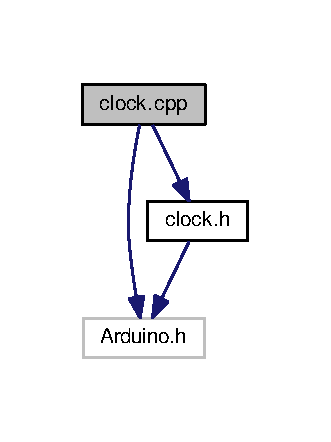
\includegraphics[width=159pt]{clock_8cpp__incl}
\end{center}
\end{figure}

\hypertarget{clock_8h}{\section{clock.\-h File Reference}
\label{clock_8h}\index{clock.\-h@{clock.\-h}}
}
{\ttfamily \#include \char`\"{}Arduino.\-h\char`\"{}}\\*
Include dependency graph for clock.\-h\-:\nopagebreak
\begin{figure}[H]
\begin{center}
\leavevmode
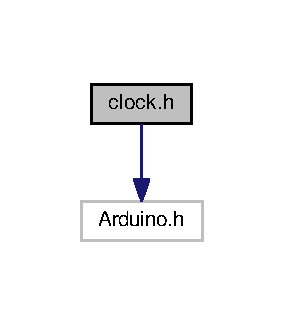
\includegraphics[width=136pt]{clock_8h__incl}
\end{center}
\end{figure}
This graph shows which files directly or indirectly include this file\-:\nopagebreak
\begin{figure}[H]
\begin{center}
\leavevmode
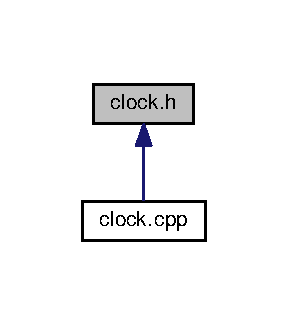
\includegraphics[width=138pt]{clock_8h__dep__incl}
\end{center}
\end{figure}
\subsection*{Classes}
\begin{DoxyCompactItemize}
\item 
class \hyperlink{classClock}{Clock}
\end{DoxyCompactItemize}
\subsection*{Enumerations}
\begin{DoxyCompactItemize}
\item 
enum \hyperlink{clock_8h_ade673c43995dab2f90ea5af75c33a83c}{e\-\_\-states} \{ \\*
\hyperlink{clock_8h_ade673c43995dab2f90ea5af75c33a83ca62fe6714ff73ae68f06737c0e1f5aa16}{Run}, 
\hyperlink{clock_8h_ade673c43995dab2f90ea5af75c33a83cabd5f9c956752ce4dc707b4624b3a36f7}{Start}, 
\hyperlink{clock_8h_ade673c43995dab2f90ea5af75c33a83ca3e85c2379b8c2d5a0a32e0eb7cec0c7d}{Restart}, 
\hyperlink{clock_8h_ade673c43995dab2f90ea5af75c33a83caf98d707eb4ed173ccfdbaf4eaa87100d}{Stop}, 
\\*
\hyperlink{clock_8h_ade673c43995dab2f90ea5af75c33a83cadaba8aa0fcd8a87c25fec7d916c789e7}{Pause}, 
\hyperlink{clock_8h_ade673c43995dab2f90ea5af75c33a83ca92793663441ced378f4676b8a6524385}{Reset}
 \}
\item 
enum \hyperlink{clock_8h_abef803757dd9b7a2b0dc5056d76d7937}{e\-\_\-mode} \{ \hyperlink{clock_8h_abef803757dd9b7a2b0dc5056d76d7937ae204c9c3e62b1e9a6b60e40cd05256c5}{Forward}, 
\hyperlink{clock_8h_abef803757dd9b7a2b0dc5056d76d7937a67e19347f85332c3bbfd61266cecbe4e}{Backward}, 
\hyperlink{clock_8h_abef803757dd9b7a2b0dc5056d76d7937ac2ba4c3e926a5fbb0304d67f047c3601}{Pendulum}, 
\hyperlink{clock_8h_abef803757dd9b7a2b0dc5056d76d7937a73610a7c860f763790e533887a479868}{Random}
 \}
\end{DoxyCompactItemize}


\subsection{Enumeration Type Documentation}
\hypertarget{clock_8h_abef803757dd9b7a2b0dc5056d76d7937}{\index{clock.\-h@{clock.\-h}!e\-\_\-mode@{e\-\_\-mode}}
\index{e\-\_\-mode@{e\-\_\-mode}!clock.h@{clock.\-h}}
\subsubsection[{e\-\_\-mode}]{\setlength{\rightskip}{0pt plus 5cm}enum {\bf e\-\_\-mode}}}\label{clock_8h_abef803757dd9b7a2b0dc5056d76d7937}
\begin{Desc}
\item[Enumerator]\par
\begin{description}
\index{Forward@{Forward}!clock.\-h@{clock.\-h}}\index{clock.\-h@{clock.\-h}!Forward@{Forward}}\item[{\em 
\hypertarget{clock_8h_abef803757dd9b7a2b0dc5056d76d7937ae204c9c3e62b1e9a6b60e40cd05256c5}{Forward}\label{clock_8h_abef803757dd9b7a2b0dc5056d76d7937ae204c9c3e62b1e9a6b60e40cd05256c5}
}]\index{Backward@{Backward}!clock.\-h@{clock.\-h}}\index{clock.\-h@{clock.\-h}!Backward@{Backward}}\item[{\em 
\hypertarget{clock_8h_abef803757dd9b7a2b0dc5056d76d7937a67e19347f85332c3bbfd61266cecbe4e}{Backward}\label{clock_8h_abef803757dd9b7a2b0dc5056d76d7937a67e19347f85332c3bbfd61266cecbe4e}
}]\index{Pendulum@{Pendulum}!clock.\-h@{clock.\-h}}\index{clock.\-h@{clock.\-h}!Pendulum@{Pendulum}}\item[{\em 
\hypertarget{clock_8h_abef803757dd9b7a2b0dc5056d76d7937ac2ba4c3e926a5fbb0304d67f047c3601}{Pendulum}\label{clock_8h_abef803757dd9b7a2b0dc5056d76d7937ac2ba4c3e926a5fbb0304d67f047c3601}
}]\index{Random@{Random}!clock.\-h@{clock.\-h}}\index{clock.\-h@{clock.\-h}!Random@{Random}}\item[{\em 
\hypertarget{clock_8h_abef803757dd9b7a2b0dc5056d76d7937a73610a7c860f763790e533887a479868}{Random}\label{clock_8h_abef803757dd9b7a2b0dc5056d76d7937a73610a7c860f763790e533887a479868}
}]\end{description}
\end{Desc}
\hypertarget{clock_8h_ade673c43995dab2f90ea5af75c33a83c}{\index{clock.\-h@{clock.\-h}!e\-\_\-states@{e\-\_\-states}}
\index{e\-\_\-states@{e\-\_\-states}!clock.h@{clock.\-h}}
\subsubsection[{e\-\_\-states}]{\setlength{\rightskip}{0pt plus 5cm}enum {\bf e\-\_\-states}}}\label{clock_8h_ade673c43995dab2f90ea5af75c33a83c}
\begin{Desc}
\item[Enumerator]\par
\begin{description}
\index{Run@{Run}!clock.\-h@{clock.\-h}}\index{clock.\-h@{clock.\-h}!Run@{Run}}\item[{\em 
\hypertarget{clock_8h_ade673c43995dab2f90ea5af75c33a83ca62fe6714ff73ae68f06737c0e1f5aa16}{Run}\label{clock_8h_ade673c43995dab2f90ea5af75c33a83ca62fe6714ff73ae68f06737c0e1f5aa16}
}]\index{Start@{Start}!clock.\-h@{clock.\-h}}\index{clock.\-h@{clock.\-h}!Start@{Start}}\item[{\em 
\hypertarget{clock_8h_ade673c43995dab2f90ea5af75c33a83cabd5f9c956752ce4dc707b4624b3a36f7}{Start}\label{clock_8h_ade673c43995dab2f90ea5af75c33a83cabd5f9c956752ce4dc707b4624b3a36f7}
}]\index{Restart@{Restart}!clock.\-h@{clock.\-h}}\index{clock.\-h@{clock.\-h}!Restart@{Restart}}\item[{\em 
\hypertarget{clock_8h_ade673c43995dab2f90ea5af75c33a83ca3e85c2379b8c2d5a0a32e0eb7cec0c7d}{Restart}\label{clock_8h_ade673c43995dab2f90ea5af75c33a83ca3e85c2379b8c2d5a0a32e0eb7cec0c7d}
}]\index{Stop@{Stop}!clock.\-h@{clock.\-h}}\index{clock.\-h@{clock.\-h}!Stop@{Stop}}\item[{\em 
\hypertarget{clock_8h_ade673c43995dab2f90ea5af75c33a83caf98d707eb4ed173ccfdbaf4eaa87100d}{Stop}\label{clock_8h_ade673c43995dab2f90ea5af75c33a83caf98d707eb4ed173ccfdbaf4eaa87100d}
}]\index{Pause@{Pause}!clock.\-h@{clock.\-h}}\index{clock.\-h@{clock.\-h}!Pause@{Pause}}\item[{\em 
\hypertarget{clock_8h_ade673c43995dab2f90ea5af75c33a83cadaba8aa0fcd8a87c25fec7d916c789e7}{Pause}\label{clock_8h_ade673c43995dab2f90ea5af75c33a83cadaba8aa0fcd8a87c25fec7d916c789e7}
}]\index{Reset@{Reset}!clock.\-h@{clock.\-h}}\index{clock.\-h@{clock.\-h}!Reset@{Reset}}\item[{\em 
\hypertarget{clock_8h_ade673c43995dab2f90ea5af75c33a83ca92793663441ced378f4676b8a6524385}{Reset}\label{clock_8h_ade673c43995dab2f90ea5af75c33a83ca92793663441ced378f4676b8a6524385}
}]\end{description}
\end{Desc}

\hypertarget{config_8h}{\section{config.\-h File Reference}
\label{config_8h}\index{config.\-h@{config.\-h}}
}
{\ttfamily \#include \char`\"{}porthardware.\-h\char`\"{}}\\*
Include dependency graph for config.\-h\-:\nopagebreak
\begin{figure}[H]
\begin{center}
\leavevmode
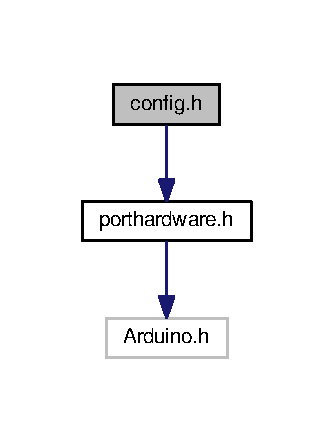
\includegraphics[width=160pt]{config_8h__incl}
\end{center}
\end{figure}
\subsection*{Macros}
\begin{DoxyCompactItemize}
\item 
\#define \hyperlink{config_8h_a60cea36aaa82fcfdb1f84a283ecbfdab}{U\-S\-E\-P\-O\-R\-T\-S}
\end{DoxyCompactItemize}


\subsection{Macro Definition Documentation}
\hypertarget{config_8h_a60cea36aaa82fcfdb1f84a283ecbfdab}{\index{config.\-h@{config.\-h}!U\-S\-E\-P\-O\-R\-T\-S@{U\-S\-E\-P\-O\-R\-T\-S}}
\index{U\-S\-E\-P\-O\-R\-T\-S@{U\-S\-E\-P\-O\-R\-T\-S}!config.h@{config.\-h}}
\subsubsection[{U\-S\-E\-P\-O\-R\-T\-S}]{\setlength{\rightskip}{0pt plus 5cm}\#define U\-S\-E\-P\-O\-R\-T\-S}}\label{config_8h_a60cea36aaa82fcfdb1f84a283ecbfdab}

\hypertarget{debug_8h}{\section{debug.\-h File Reference}
\label{debug_8h}\index{debug.\-h@{debug.\-h}}
}
This graph shows which files directly or indirectly include this file\-:
\nopagebreak
\begin{figure}[H]
\begin{center}
\leavevmode
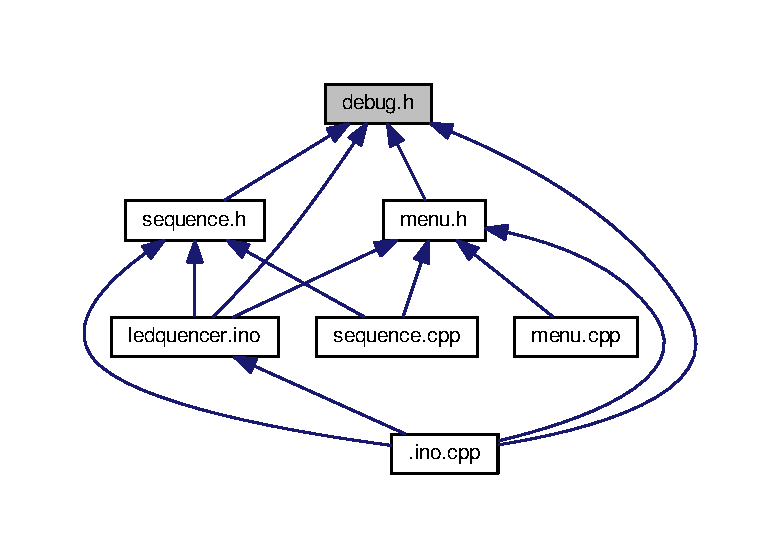
\includegraphics[width=350pt]{debug_8h__dep__incl}
\end{center}
\end{figure}
\subsection*{Macros}
\begin{DoxyCompactItemize}
\item 
\#define \hyperlink{debug_8h_a3dfa58b1c5c2943dd49d8aa1981d377d}{D\-E\-B\-U\-G}(x)~do \{if (\hyperlink{ledquencer_8ino_a0f5109855ecd58cd3b97d093ac9815f2}{debugging\-\_\-enabled}) \{ Serial.\-println(x);\}\} while (0)
\end{DoxyCompactItemize}
\subsection*{Variables}
\begin{DoxyCompactItemize}
\item 
int \hyperlink{debug_8h_a0f5109855ecd58cd3b97d093ac9815f2}{debugging\-\_\-enabled}
\end{DoxyCompactItemize}


\subsection{Macro Definition Documentation}
\hypertarget{debug_8h_a3dfa58b1c5c2943dd49d8aa1981d377d}{\index{debug.\-h@{debug.\-h}!D\-E\-B\-U\-G@{D\-E\-B\-U\-G}}
\index{D\-E\-B\-U\-G@{D\-E\-B\-U\-G}!debug.h@{debug.\-h}}
\subsubsection[{D\-E\-B\-U\-G}]{\setlength{\rightskip}{0pt plus 5cm}\#define D\-E\-B\-U\-G(
\begin{DoxyParamCaption}
\item[{}]{x}
\end{DoxyParamCaption}
)~do \{if ({\bf debugging\-\_\-enabled}) \{ Serial.\-println(x);\}\} while (0)}}\label{debug_8h_a3dfa58b1c5c2943dd49d8aa1981d377d}


\subsection{Variable Documentation}
\hypertarget{debug_8h_a0f5109855ecd58cd3b97d093ac9815f2}{\index{debug.\-h@{debug.\-h}!debugging\-\_\-enabled@{debugging\-\_\-enabled}}
\index{debugging\-\_\-enabled@{debugging\-\_\-enabled}!debug.h@{debug.\-h}}
\subsubsection[{debugging\-\_\-enabled}]{\setlength{\rightskip}{0pt plus 5cm}int debugging\-\_\-enabled}}\label{debug_8h_a0f5109855ecd58cd3b97d093ac9815f2}

\hypertarget{funcs_8cpp}{\section{funcs.\-cpp File Reference}
\label{funcs_8cpp}\index{funcs.\-cpp@{funcs.\-cpp}}
}
{\ttfamily \#include \char`\"{}funcs.\-h\char`\"{}}\\*
Include dependency graph for funcs.\-cpp\-:\nopagebreak
\begin{figure}[H]
\begin{center}
\leavevmode
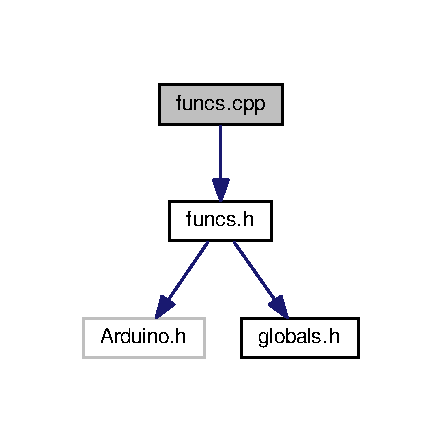
\includegraphics[width=212pt]{funcs_8cpp__incl}
\end{center}
\end{figure}
\subsection*{Functions}
\begin{DoxyCompactItemize}
\item 
bool \hyperlink{funcs_8cpp_a570af57b9b56e8d48da6b6ee3b8b8c4e}{debounce} (bool akt, int statenr)
\end{DoxyCompactItemize}


\subsection{Function Documentation}
\hypertarget{funcs_8cpp_a570af57b9b56e8d48da6b6ee3b8b8c4e}{\index{funcs.\-cpp@{funcs.\-cpp}!debounce@{debounce}}
\index{debounce@{debounce}!funcs.cpp@{funcs.\-cpp}}
\subsubsection[{debounce}]{\setlength{\rightskip}{0pt plus 5cm}bool debounce (
\begin{DoxyParamCaption}
\item[{bool}]{akt, }
\item[{int}]{statenr}
\end{DoxyParamCaption}
)\hspace{0.3cm}{\ttfamily [inline]}}}\label{funcs_8cpp_a570af57b9b56e8d48da6b6ee3b8b8c4e}

\hypertarget{funcs_8h}{\section{funcs.\-h File Reference}
\label{funcs_8h}\index{funcs.\-h@{funcs.\-h}}
}
{\ttfamily \#include $<$Arduino.\-h$>$}\\*
{\ttfamily \#include \char`\"{}globals.\-h\char`\"{}}\\*
Include dependency graph for funcs.\-h\-:\nopagebreak
\begin{figure}[H]
\begin{center}
\leavevmode
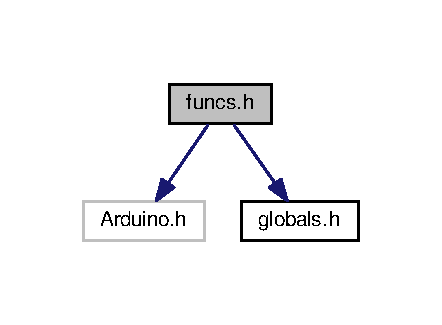
\includegraphics[width=212pt]{funcs_8h__incl}
\end{center}
\end{figure}
This graph shows which files directly or indirectly include this file\-:\nopagebreak
\begin{figure}[H]
\begin{center}
\leavevmode
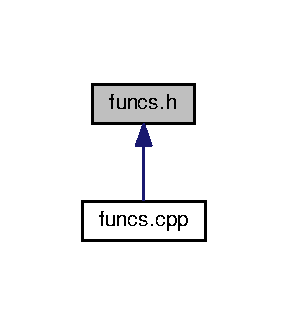
\includegraphics[width=138pt]{funcs_8h__dep__incl}
\end{center}
\end{figure}
\subsection*{Functions}
\begin{DoxyCompactItemize}
\item 
bool \hyperlink{funcs_8h_a9a059537769fa317e5574271ded2819d}{debounce} (bool, int)
\end{DoxyCompactItemize}


\subsection{Function Documentation}
\hypertarget{funcs_8h_a9a059537769fa317e5574271ded2819d}{\index{funcs.\-h@{funcs.\-h}!debounce@{debounce}}
\index{debounce@{debounce}!funcs.h@{funcs.\-h}}
\subsubsection[{debounce}]{\setlength{\rightskip}{0pt plus 5cm}bool debounce (
\begin{DoxyParamCaption}
\item[{bool}]{, }
\item[{int}]{}
\end{DoxyParamCaption}
)\hspace{0.3cm}{\ttfamily [inline]}}}\label{funcs_8h_a9a059537769fa317e5574271ded2819d}

\hypertarget{globals_8h}{\section{globals.\-h File Reference}
\label{globals_8h}\index{globals.\-h@{globals.\-h}}
}
This graph shows which files directly or indirectly include this file\-:
\nopagebreak
\begin{figure}[H]
\begin{center}
\leavevmode
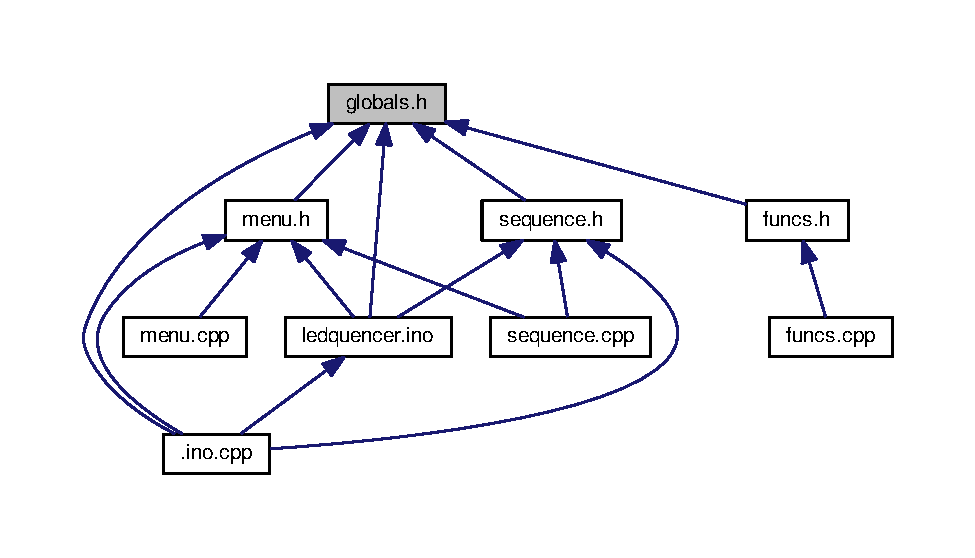
\includegraphics[width=350pt]{globals_8h__dep__incl}
\end{center}
\end{figure}
\subsection*{Macros}
\begin{DoxyCompactItemize}
\item 
\#define \hyperlink{globals_8h_a956190b59cb29810a23d34a2aefa4a21}{P\-A\-T\-L\-E\-N}~16
\item 
\#define \hyperlink{globals_8h_ae720886adf10f6a72983c7b2341cf0a3}{T\-R\-A\-C\-K\-S}~16
\item 
\#define \hyperlink{globals_8h_a1e7d540f56d5bfa784fa9dd8286347d7}{Tout01}~26
\item 
\#define \hyperlink{globals_8h_ab26d31c7d698e28ac758d2c768fbf49a}{Tout02}~25
\item 
\#define \hyperlink{globals_8h_ab19e5d3e16c5a8775de47c1f8c08bdc8}{Tout03}~24
\item 
\#define \hyperlink{globals_8h_aa9594bf2eee1c426b5d470b6934daf87}{Tout04}~23
\item 
\#define \hyperlink{globals_8h_ad20eacd4271934867e047a3a58e721d3}{Tout05}~22
\item 
\#define \hyperlink{globals_8h_a9e5126c4734b6d53ac1ba81d8acf8c5e}{Tout06}~2
\item 
\#define \hyperlink{globals_8h_a7be59ae745ad59d186c223e4620571c2}{Tout07}~3
\item 
\#define \hyperlink{globals_8h_ae85d0126caf8dc7616a48129b8bac8e8}{Tout08}~4
\item 
\#define \hyperlink{globals_8h_a448dcd3cee8c2f9c07122530429f2cee}{Tout09}~5
\item 
\#define \hyperlink{globals_8h_ae2125172b37fe080035bc537d4d3c351}{Tout10}~6
\item 
\#define \hyperlink{globals_8h_a9abeefbf4cbeda1bcb9727a41595947e}{Tout11}~7
\item 
\#define \hyperlink{globals_8h_a95587f997bf9a350ffdcd8e6fbc8508d}{Tout12}~8
\item 
\#define \hyperlink{globals_8h_a973369a7421d6b3c0bd785482b6c1c3c}{Tout13}~9
\item 
\#define \hyperlink{globals_8h_a348ed2963d95416f7f3584b3f4fe5e8f}{Tout14}~10
\item 
\#define \hyperlink{globals_8h_ac49e072ebe0c09d9a60add72d5c03f82}{Tout15}~11
\item 
\#define \hyperlink{globals_8h_aaf450ad080f1921bc6d6fe37968a2c92}{Tout16}~12
\item 
\#define \hyperlink{globals_8h_ab05d2adb8967ade26a215b2cc84fecb7}{clkout}~27
\item 
\#define \hyperlink{globals_8h_a4d15208cf1c774120448484c40ff6904}{clkin}~28
\item 
\#define \hyperlink{globals_8h_a14a83d16a4531a8b9b80ced3ce4fbbca}{midiout}~1
\item 
\#define \hyperlink{globals_8h_a01ddc83527d9721893f4672c413054d9}{midiin}~0
\item 
\#define \hyperlink{globals_8h_abc485487ee5251eec157c5ad0bb796cb}{mux1\-A0}~35
\item 
\#define \hyperlink{globals_8h_a249002e36cc1ab40c44ac27820fae78f}{mux1\-A1}~36
\item 
\#define \hyperlink{globals_8h_a2bc2f0212bd88c42f887c0db759dc339}{mux1\-A2}~33
\item 
\#define \hyperlink{globals_8h_af06bcad0352cf0124ba905197669f8e4}{mux1\-A3}~34
\item 
\#define \hyperlink{globals_8h_a10a7aab4f9cc1c3489fb97bf895a8490}{mux2\-A0}~37
\item 
\#define \hyperlink{globals_8h_af199c836e1afbe7001520ee1f44ccad2}{mux2\-A1}~38
\item 
\#define \hyperlink{globals_8h_a885ded37ec54b0498883db24c2276666}{mux2\-A2}~31
\item 
\#define \hyperlink{globals_8h_a85b3f73148c31d0ca64b2d9099e50a7f}{mux2\-A3}~32
\item 
\#define \hyperlink{globals_8h_a1fde236889c6f4697462c7a41c9796fc}{mux3\-A0}~39
\item 
\#define \hyperlink{globals_8h_a04bc247f8a5df32cee502f156d8d6230}{mux3\-A1}~40
\item 
\#define \hyperlink{globals_8h_a22da0292e2bc8defee00df32d3aa84c5}{mux3\-A2}~30
\item 
\#define \hyperlink{globals_8h_a2014d86e5cfd73354a1a2ba880072191}{mux3\-A3}~29
\item 
\#define \hyperlink{globals_8h_af0d5f8bf5ce884b44d4da65910b9599d}{muxlatch}~41
\item 
\#define \hyperlink{globals_8h_a8277ab199bfff2a2b9e59af826663b2b}{S\-B01}~A1
\item 
\#define \hyperlink{globals_8h_add6ae2e78aba0310a54b20e9308b720e}{S\-B02}~A3
\item 
\#define \hyperlink{globals_8h_a6a597f9c7295d685eef049f859bf0e30}{S\-B03}~A5
\item 
\#define \hyperlink{globals_8h_a808ebefbb07fd08e5833eb661a5a5133}{S\-B04}~A7
\item 
\#define \hyperlink{globals_8h_a8e716449378b744a873473e898ea8156}{S\-B05}~A9
\item 
\#define \hyperlink{globals_8h_aaea67207de0f9f63ac6f623cc9dbfda6}{S\-B06}~A11
\item 
\#define \hyperlink{globals_8h_ab7037137e82d427ed9b3c39480f95b0c}{S\-B07}~53
\item 
\#define \hyperlink{globals_8h_a444c4da3e4cc7e814a660881720d2fde}{S\-B08}~51
\item 
\#define \hyperlink{globals_8h_a3f7d0c6ac8995ae0db6e1fe3e9c9d978}{S\-B09}~49
\item 
\#define \hyperlink{globals_8h_a002d444aca24117e132bbeda2c640b8e}{S\-B10}~47
\item 
\#define \hyperlink{globals_8h_a5b67ad1cde93cb1e0801563a910ad293}{S\-B11}~45
\item 
\#define \hyperlink{globals_8h_a073bed928178eec0ef1a93190d7eb346}{S\-B12}~43
\item 
\#define \hyperlink{globals_8h_a474dac268e92be6058111137c2699820}{S\-B13}~48
\item 
\#define \hyperlink{globals_8h_a1af2e241031fcc38769499396855033c}{S\-B14}~46
\item 
\#define \hyperlink{globals_8h_ab7486af29915b0d6dfd40fa4453f03bf}{S\-B15}~44
\item 
\#define \hyperlink{globals_8h_ac2f3c425bdd1a2f76c6afbbf4fa802b8}{S\-B16}~42
\item 
\#define \hyperlink{globals_8h_a065a4a815bdaefcd4abc0ebf5fed76a7}{F\-B01}~A0
\item 
\#define \hyperlink{globals_8h_afc532eee7ba794f9ccfa9b4d4e3487d7}{F\-B02}~A2
\item 
\#define \hyperlink{globals_8h_aeb65683e3b3a9b8885cab1dccf075a19}{F\-B03}~A4
\item 
\#define \hyperlink{globals_8h_a1d08cbf55764cf56ec94ba758c2647fc}{F\-B04}~A6
\item 
\#define \hyperlink{globals_8h_aa287e9bad467a3a1dccfdf056c0c633d}{F\-B05}~A8
\item 
\#define \hyperlink{globals_8h_a906386975c352e480a7e119057017062}{F\-B06}~A10
\item 
\#define \hyperlink{globals_8h_af5e0e9e8adf066feb38f1bde8197dfc5}{F\-B07}~52
\item 
\#define \hyperlink{globals_8h_a6c5d2587d6ea4a9f5b56fe83830b2cf2}{F\-B08}~50
\end{DoxyCompactItemize}


\subsection{Macro Definition Documentation}
\hypertarget{globals_8h_a4d15208cf1c774120448484c40ff6904}{\index{globals.\-h@{globals.\-h}!clkin@{clkin}}
\index{clkin@{clkin}!globals.h@{globals.\-h}}
\subsubsection[{clkin}]{\setlength{\rightskip}{0pt plus 5cm}\#define clkin~28}}\label{globals_8h_a4d15208cf1c774120448484c40ff6904}
\hypertarget{globals_8h_ab05d2adb8967ade26a215b2cc84fecb7}{\index{globals.\-h@{globals.\-h}!clkout@{clkout}}
\index{clkout@{clkout}!globals.h@{globals.\-h}}
\subsubsection[{clkout}]{\setlength{\rightskip}{0pt plus 5cm}\#define clkout~27}}\label{globals_8h_ab05d2adb8967ade26a215b2cc84fecb7}
\hypertarget{globals_8h_a065a4a815bdaefcd4abc0ebf5fed76a7}{\index{globals.\-h@{globals.\-h}!F\-B01@{F\-B01}}
\index{F\-B01@{F\-B01}!globals.h@{globals.\-h}}
\subsubsection[{F\-B01}]{\setlength{\rightskip}{0pt plus 5cm}\#define F\-B01~A0}}\label{globals_8h_a065a4a815bdaefcd4abc0ebf5fed76a7}
\hypertarget{globals_8h_afc532eee7ba794f9ccfa9b4d4e3487d7}{\index{globals.\-h@{globals.\-h}!F\-B02@{F\-B02}}
\index{F\-B02@{F\-B02}!globals.h@{globals.\-h}}
\subsubsection[{F\-B02}]{\setlength{\rightskip}{0pt plus 5cm}\#define F\-B02~A2}}\label{globals_8h_afc532eee7ba794f9ccfa9b4d4e3487d7}
\hypertarget{globals_8h_aeb65683e3b3a9b8885cab1dccf075a19}{\index{globals.\-h@{globals.\-h}!F\-B03@{F\-B03}}
\index{F\-B03@{F\-B03}!globals.h@{globals.\-h}}
\subsubsection[{F\-B03}]{\setlength{\rightskip}{0pt plus 5cm}\#define F\-B03~A4}}\label{globals_8h_aeb65683e3b3a9b8885cab1dccf075a19}
\hypertarget{globals_8h_a1d08cbf55764cf56ec94ba758c2647fc}{\index{globals.\-h@{globals.\-h}!F\-B04@{F\-B04}}
\index{F\-B04@{F\-B04}!globals.h@{globals.\-h}}
\subsubsection[{F\-B04}]{\setlength{\rightskip}{0pt plus 5cm}\#define F\-B04~A6}}\label{globals_8h_a1d08cbf55764cf56ec94ba758c2647fc}
\hypertarget{globals_8h_aa287e9bad467a3a1dccfdf056c0c633d}{\index{globals.\-h@{globals.\-h}!F\-B05@{F\-B05}}
\index{F\-B05@{F\-B05}!globals.h@{globals.\-h}}
\subsubsection[{F\-B05}]{\setlength{\rightskip}{0pt plus 5cm}\#define F\-B05~A8}}\label{globals_8h_aa287e9bad467a3a1dccfdf056c0c633d}
\hypertarget{globals_8h_a906386975c352e480a7e119057017062}{\index{globals.\-h@{globals.\-h}!F\-B06@{F\-B06}}
\index{F\-B06@{F\-B06}!globals.h@{globals.\-h}}
\subsubsection[{F\-B06}]{\setlength{\rightskip}{0pt plus 5cm}\#define F\-B06~A10}}\label{globals_8h_a906386975c352e480a7e119057017062}
\hypertarget{globals_8h_af5e0e9e8adf066feb38f1bde8197dfc5}{\index{globals.\-h@{globals.\-h}!F\-B07@{F\-B07}}
\index{F\-B07@{F\-B07}!globals.h@{globals.\-h}}
\subsubsection[{F\-B07}]{\setlength{\rightskip}{0pt plus 5cm}\#define F\-B07~52}}\label{globals_8h_af5e0e9e8adf066feb38f1bde8197dfc5}
\hypertarget{globals_8h_a6c5d2587d6ea4a9f5b56fe83830b2cf2}{\index{globals.\-h@{globals.\-h}!F\-B08@{F\-B08}}
\index{F\-B08@{F\-B08}!globals.h@{globals.\-h}}
\subsubsection[{F\-B08}]{\setlength{\rightskip}{0pt plus 5cm}\#define F\-B08~50}}\label{globals_8h_a6c5d2587d6ea4a9f5b56fe83830b2cf2}
\hypertarget{globals_8h_a01ddc83527d9721893f4672c413054d9}{\index{globals.\-h@{globals.\-h}!midiin@{midiin}}
\index{midiin@{midiin}!globals.h@{globals.\-h}}
\subsubsection[{midiin}]{\setlength{\rightskip}{0pt plus 5cm}\#define midiin~0}}\label{globals_8h_a01ddc83527d9721893f4672c413054d9}
\hypertarget{globals_8h_a14a83d16a4531a8b9b80ced3ce4fbbca}{\index{globals.\-h@{globals.\-h}!midiout@{midiout}}
\index{midiout@{midiout}!globals.h@{globals.\-h}}
\subsubsection[{midiout}]{\setlength{\rightskip}{0pt plus 5cm}\#define midiout~1}}\label{globals_8h_a14a83d16a4531a8b9b80ced3ce4fbbca}
\hypertarget{globals_8h_abc485487ee5251eec157c5ad0bb796cb}{\index{globals.\-h@{globals.\-h}!mux1\-A0@{mux1\-A0}}
\index{mux1\-A0@{mux1\-A0}!globals.h@{globals.\-h}}
\subsubsection[{mux1\-A0}]{\setlength{\rightskip}{0pt plus 5cm}\#define mux1\-A0~35}}\label{globals_8h_abc485487ee5251eec157c5ad0bb796cb}
\hypertarget{globals_8h_a249002e36cc1ab40c44ac27820fae78f}{\index{globals.\-h@{globals.\-h}!mux1\-A1@{mux1\-A1}}
\index{mux1\-A1@{mux1\-A1}!globals.h@{globals.\-h}}
\subsubsection[{mux1\-A1}]{\setlength{\rightskip}{0pt plus 5cm}\#define mux1\-A1~36}}\label{globals_8h_a249002e36cc1ab40c44ac27820fae78f}
\hypertarget{globals_8h_a2bc2f0212bd88c42f887c0db759dc339}{\index{globals.\-h@{globals.\-h}!mux1\-A2@{mux1\-A2}}
\index{mux1\-A2@{mux1\-A2}!globals.h@{globals.\-h}}
\subsubsection[{mux1\-A2}]{\setlength{\rightskip}{0pt plus 5cm}\#define mux1\-A2~33}}\label{globals_8h_a2bc2f0212bd88c42f887c0db759dc339}
\hypertarget{globals_8h_af06bcad0352cf0124ba905197669f8e4}{\index{globals.\-h@{globals.\-h}!mux1\-A3@{mux1\-A3}}
\index{mux1\-A3@{mux1\-A3}!globals.h@{globals.\-h}}
\subsubsection[{mux1\-A3}]{\setlength{\rightskip}{0pt plus 5cm}\#define mux1\-A3~34}}\label{globals_8h_af06bcad0352cf0124ba905197669f8e4}
\hypertarget{globals_8h_a10a7aab4f9cc1c3489fb97bf895a8490}{\index{globals.\-h@{globals.\-h}!mux2\-A0@{mux2\-A0}}
\index{mux2\-A0@{mux2\-A0}!globals.h@{globals.\-h}}
\subsubsection[{mux2\-A0}]{\setlength{\rightskip}{0pt plus 5cm}\#define mux2\-A0~37}}\label{globals_8h_a10a7aab4f9cc1c3489fb97bf895a8490}
\hypertarget{globals_8h_af199c836e1afbe7001520ee1f44ccad2}{\index{globals.\-h@{globals.\-h}!mux2\-A1@{mux2\-A1}}
\index{mux2\-A1@{mux2\-A1}!globals.h@{globals.\-h}}
\subsubsection[{mux2\-A1}]{\setlength{\rightskip}{0pt plus 5cm}\#define mux2\-A1~38}}\label{globals_8h_af199c836e1afbe7001520ee1f44ccad2}
\hypertarget{globals_8h_a885ded37ec54b0498883db24c2276666}{\index{globals.\-h@{globals.\-h}!mux2\-A2@{mux2\-A2}}
\index{mux2\-A2@{mux2\-A2}!globals.h@{globals.\-h}}
\subsubsection[{mux2\-A2}]{\setlength{\rightskip}{0pt plus 5cm}\#define mux2\-A2~31}}\label{globals_8h_a885ded37ec54b0498883db24c2276666}
\hypertarget{globals_8h_a85b3f73148c31d0ca64b2d9099e50a7f}{\index{globals.\-h@{globals.\-h}!mux2\-A3@{mux2\-A3}}
\index{mux2\-A3@{mux2\-A3}!globals.h@{globals.\-h}}
\subsubsection[{mux2\-A3}]{\setlength{\rightskip}{0pt plus 5cm}\#define mux2\-A3~32}}\label{globals_8h_a85b3f73148c31d0ca64b2d9099e50a7f}
\hypertarget{globals_8h_a1fde236889c6f4697462c7a41c9796fc}{\index{globals.\-h@{globals.\-h}!mux3\-A0@{mux3\-A0}}
\index{mux3\-A0@{mux3\-A0}!globals.h@{globals.\-h}}
\subsubsection[{mux3\-A0}]{\setlength{\rightskip}{0pt plus 5cm}\#define mux3\-A0~39}}\label{globals_8h_a1fde236889c6f4697462c7a41c9796fc}
\hypertarget{globals_8h_a04bc247f8a5df32cee502f156d8d6230}{\index{globals.\-h@{globals.\-h}!mux3\-A1@{mux3\-A1}}
\index{mux3\-A1@{mux3\-A1}!globals.h@{globals.\-h}}
\subsubsection[{mux3\-A1}]{\setlength{\rightskip}{0pt plus 5cm}\#define mux3\-A1~40}}\label{globals_8h_a04bc247f8a5df32cee502f156d8d6230}
\hypertarget{globals_8h_a22da0292e2bc8defee00df32d3aa84c5}{\index{globals.\-h@{globals.\-h}!mux3\-A2@{mux3\-A2}}
\index{mux3\-A2@{mux3\-A2}!globals.h@{globals.\-h}}
\subsubsection[{mux3\-A2}]{\setlength{\rightskip}{0pt plus 5cm}\#define mux3\-A2~30}}\label{globals_8h_a22da0292e2bc8defee00df32d3aa84c5}
\hypertarget{globals_8h_a2014d86e5cfd73354a1a2ba880072191}{\index{globals.\-h@{globals.\-h}!mux3\-A3@{mux3\-A3}}
\index{mux3\-A3@{mux3\-A3}!globals.h@{globals.\-h}}
\subsubsection[{mux3\-A3}]{\setlength{\rightskip}{0pt plus 5cm}\#define mux3\-A3~29}}\label{globals_8h_a2014d86e5cfd73354a1a2ba880072191}
\hypertarget{globals_8h_af0d5f8bf5ce884b44d4da65910b9599d}{\index{globals.\-h@{globals.\-h}!muxlatch@{muxlatch}}
\index{muxlatch@{muxlatch}!globals.h@{globals.\-h}}
\subsubsection[{muxlatch}]{\setlength{\rightskip}{0pt plus 5cm}\#define muxlatch~41}}\label{globals_8h_af0d5f8bf5ce884b44d4da65910b9599d}
\hypertarget{globals_8h_a956190b59cb29810a23d34a2aefa4a21}{\index{globals.\-h@{globals.\-h}!P\-A\-T\-L\-E\-N@{P\-A\-T\-L\-E\-N}}
\index{P\-A\-T\-L\-E\-N@{P\-A\-T\-L\-E\-N}!globals.h@{globals.\-h}}
\subsubsection[{P\-A\-T\-L\-E\-N}]{\setlength{\rightskip}{0pt plus 5cm}\#define P\-A\-T\-L\-E\-N~16}}\label{globals_8h_a956190b59cb29810a23d34a2aefa4a21}
\hypertarget{globals_8h_a8277ab199bfff2a2b9e59af826663b2b}{\index{globals.\-h@{globals.\-h}!S\-B01@{S\-B01}}
\index{S\-B01@{S\-B01}!globals.h@{globals.\-h}}
\subsubsection[{S\-B01}]{\setlength{\rightskip}{0pt plus 5cm}\#define S\-B01~A1}}\label{globals_8h_a8277ab199bfff2a2b9e59af826663b2b}
\hypertarget{globals_8h_add6ae2e78aba0310a54b20e9308b720e}{\index{globals.\-h@{globals.\-h}!S\-B02@{S\-B02}}
\index{S\-B02@{S\-B02}!globals.h@{globals.\-h}}
\subsubsection[{S\-B02}]{\setlength{\rightskip}{0pt plus 5cm}\#define S\-B02~A3}}\label{globals_8h_add6ae2e78aba0310a54b20e9308b720e}
\hypertarget{globals_8h_a6a597f9c7295d685eef049f859bf0e30}{\index{globals.\-h@{globals.\-h}!S\-B03@{S\-B03}}
\index{S\-B03@{S\-B03}!globals.h@{globals.\-h}}
\subsubsection[{S\-B03}]{\setlength{\rightskip}{0pt plus 5cm}\#define S\-B03~A5}}\label{globals_8h_a6a597f9c7295d685eef049f859bf0e30}
\hypertarget{globals_8h_a808ebefbb07fd08e5833eb661a5a5133}{\index{globals.\-h@{globals.\-h}!S\-B04@{S\-B04}}
\index{S\-B04@{S\-B04}!globals.h@{globals.\-h}}
\subsubsection[{S\-B04}]{\setlength{\rightskip}{0pt plus 5cm}\#define S\-B04~A7}}\label{globals_8h_a808ebefbb07fd08e5833eb661a5a5133}
\hypertarget{globals_8h_a8e716449378b744a873473e898ea8156}{\index{globals.\-h@{globals.\-h}!S\-B05@{S\-B05}}
\index{S\-B05@{S\-B05}!globals.h@{globals.\-h}}
\subsubsection[{S\-B05}]{\setlength{\rightskip}{0pt plus 5cm}\#define S\-B05~A9}}\label{globals_8h_a8e716449378b744a873473e898ea8156}
\hypertarget{globals_8h_aaea67207de0f9f63ac6f623cc9dbfda6}{\index{globals.\-h@{globals.\-h}!S\-B06@{S\-B06}}
\index{S\-B06@{S\-B06}!globals.h@{globals.\-h}}
\subsubsection[{S\-B06}]{\setlength{\rightskip}{0pt plus 5cm}\#define S\-B06~A11}}\label{globals_8h_aaea67207de0f9f63ac6f623cc9dbfda6}
\hypertarget{globals_8h_ab7037137e82d427ed9b3c39480f95b0c}{\index{globals.\-h@{globals.\-h}!S\-B07@{S\-B07}}
\index{S\-B07@{S\-B07}!globals.h@{globals.\-h}}
\subsubsection[{S\-B07}]{\setlength{\rightskip}{0pt plus 5cm}\#define S\-B07~53}}\label{globals_8h_ab7037137e82d427ed9b3c39480f95b0c}
\hypertarget{globals_8h_a444c4da3e4cc7e814a660881720d2fde}{\index{globals.\-h@{globals.\-h}!S\-B08@{S\-B08}}
\index{S\-B08@{S\-B08}!globals.h@{globals.\-h}}
\subsubsection[{S\-B08}]{\setlength{\rightskip}{0pt plus 5cm}\#define S\-B08~51}}\label{globals_8h_a444c4da3e4cc7e814a660881720d2fde}
\hypertarget{globals_8h_a3f7d0c6ac8995ae0db6e1fe3e9c9d978}{\index{globals.\-h@{globals.\-h}!S\-B09@{S\-B09}}
\index{S\-B09@{S\-B09}!globals.h@{globals.\-h}}
\subsubsection[{S\-B09}]{\setlength{\rightskip}{0pt plus 5cm}\#define S\-B09~49}}\label{globals_8h_a3f7d0c6ac8995ae0db6e1fe3e9c9d978}
\hypertarget{globals_8h_a002d444aca24117e132bbeda2c640b8e}{\index{globals.\-h@{globals.\-h}!S\-B10@{S\-B10}}
\index{S\-B10@{S\-B10}!globals.h@{globals.\-h}}
\subsubsection[{S\-B10}]{\setlength{\rightskip}{0pt plus 5cm}\#define S\-B10~47}}\label{globals_8h_a002d444aca24117e132bbeda2c640b8e}
\hypertarget{globals_8h_a5b67ad1cde93cb1e0801563a910ad293}{\index{globals.\-h@{globals.\-h}!S\-B11@{S\-B11}}
\index{S\-B11@{S\-B11}!globals.h@{globals.\-h}}
\subsubsection[{S\-B11}]{\setlength{\rightskip}{0pt plus 5cm}\#define S\-B11~45}}\label{globals_8h_a5b67ad1cde93cb1e0801563a910ad293}
\hypertarget{globals_8h_a073bed928178eec0ef1a93190d7eb346}{\index{globals.\-h@{globals.\-h}!S\-B12@{S\-B12}}
\index{S\-B12@{S\-B12}!globals.h@{globals.\-h}}
\subsubsection[{S\-B12}]{\setlength{\rightskip}{0pt plus 5cm}\#define S\-B12~43}}\label{globals_8h_a073bed928178eec0ef1a93190d7eb346}
\hypertarget{globals_8h_a474dac268e92be6058111137c2699820}{\index{globals.\-h@{globals.\-h}!S\-B13@{S\-B13}}
\index{S\-B13@{S\-B13}!globals.h@{globals.\-h}}
\subsubsection[{S\-B13}]{\setlength{\rightskip}{0pt plus 5cm}\#define S\-B13~48}}\label{globals_8h_a474dac268e92be6058111137c2699820}
\hypertarget{globals_8h_a1af2e241031fcc38769499396855033c}{\index{globals.\-h@{globals.\-h}!S\-B14@{S\-B14}}
\index{S\-B14@{S\-B14}!globals.h@{globals.\-h}}
\subsubsection[{S\-B14}]{\setlength{\rightskip}{0pt plus 5cm}\#define S\-B14~46}}\label{globals_8h_a1af2e241031fcc38769499396855033c}
\hypertarget{globals_8h_ab7486af29915b0d6dfd40fa4453f03bf}{\index{globals.\-h@{globals.\-h}!S\-B15@{S\-B15}}
\index{S\-B15@{S\-B15}!globals.h@{globals.\-h}}
\subsubsection[{S\-B15}]{\setlength{\rightskip}{0pt plus 5cm}\#define S\-B15~44}}\label{globals_8h_ab7486af29915b0d6dfd40fa4453f03bf}
\hypertarget{globals_8h_ac2f3c425bdd1a2f76c6afbbf4fa802b8}{\index{globals.\-h@{globals.\-h}!S\-B16@{S\-B16}}
\index{S\-B16@{S\-B16}!globals.h@{globals.\-h}}
\subsubsection[{S\-B16}]{\setlength{\rightskip}{0pt plus 5cm}\#define S\-B16~42}}\label{globals_8h_ac2f3c425bdd1a2f76c6afbbf4fa802b8}
\hypertarget{globals_8h_a1e7d540f56d5bfa784fa9dd8286347d7}{\index{globals.\-h@{globals.\-h}!Tout01@{Tout01}}
\index{Tout01@{Tout01}!globals.h@{globals.\-h}}
\subsubsection[{Tout01}]{\setlength{\rightskip}{0pt plus 5cm}\#define Tout01~26}}\label{globals_8h_a1e7d540f56d5bfa784fa9dd8286347d7}
\hypertarget{globals_8h_ab26d31c7d698e28ac758d2c768fbf49a}{\index{globals.\-h@{globals.\-h}!Tout02@{Tout02}}
\index{Tout02@{Tout02}!globals.h@{globals.\-h}}
\subsubsection[{Tout02}]{\setlength{\rightskip}{0pt plus 5cm}\#define Tout02~25}}\label{globals_8h_ab26d31c7d698e28ac758d2c768fbf49a}
\hypertarget{globals_8h_ab19e5d3e16c5a8775de47c1f8c08bdc8}{\index{globals.\-h@{globals.\-h}!Tout03@{Tout03}}
\index{Tout03@{Tout03}!globals.h@{globals.\-h}}
\subsubsection[{Tout03}]{\setlength{\rightskip}{0pt plus 5cm}\#define Tout03~24}}\label{globals_8h_ab19e5d3e16c5a8775de47c1f8c08bdc8}
\hypertarget{globals_8h_aa9594bf2eee1c426b5d470b6934daf87}{\index{globals.\-h@{globals.\-h}!Tout04@{Tout04}}
\index{Tout04@{Tout04}!globals.h@{globals.\-h}}
\subsubsection[{Tout04}]{\setlength{\rightskip}{0pt plus 5cm}\#define Tout04~23}}\label{globals_8h_aa9594bf2eee1c426b5d470b6934daf87}
\hypertarget{globals_8h_ad20eacd4271934867e047a3a58e721d3}{\index{globals.\-h@{globals.\-h}!Tout05@{Tout05}}
\index{Tout05@{Tout05}!globals.h@{globals.\-h}}
\subsubsection[{Tout05}]{\setlength{\rightskip}{0pt plus 5cm}\#define Tout05~22}}\label{globals_8h_ad20eacd4271934867e047a3a58e721d3}
\hypertarget{globals_8h_a9e5126c4734b6d53ac1ba81d8acf8c5e}{\index{globals.\-h@{globals.\-h}!Tout06@{Tout06}}
\index{Tout06@{Tout06}!globals.h@{globals.\-h}}
\subsubsection[{Tout06}]{\setlength{\rightskip}{0pt plus 5cm}\#define Tout06~2}}\label{globals_8h_a9e5126c4734b6d53ac1ba81d8acf8c5e}
\hypertarget{globals_8h_a7be59ae745ad59d186c223e4620571c2}{\index{globals.\-h@{globals.\-h}!Tout07@{Tout07}}
\index{Tout07@{Tout07}!globals.h@{globals.\-h}}
\subsubsection[{Tout07}]{\setlength{\rightskip}{0pt plus 5cm}\#define Tout07~3}}\label{globals_8h_a7be59ae745ad59d186c223e4620571c2}
\hypertarget{globals_8h_ae85d0126caf8dc7616a48129b8bac8e8}{\index{globals.\-h@{globals.\-h}!Tout08@{Tout08}}
\index{Tout08@{Tout08}!globals.h@{globals.\-h}}
\subsubsection[{Tout08}]{\setlength{\rightskip}{0pt plus 5cm}\#define Tout08~4}}\label{globals_8h_ae85d0126caf8dc7616a48129b8bac8e8}
\hypertarget{globals_8h_a448dcd3cee8c2f9c07122530429f2cee}{\index{globals.\-h@{globals.\-h}!Tout09@{Tout09}}
\index{Tout09@{Tout09}!globals.h@{globals.\-h}}
\subsubsection[{Tout09}]{\setlength{\rightskip}{0pt plus 5cm}\#define Tout09~5}}\label{globals_8h_a448dcd3cee8c2f9c07122530429f2cee}
\hypertarget{globals_8h_ae2125172b37fe080035bc537d4d3c351}{\index{globals.\-h@{globals.\-h}!Tout10@{Tout10}}
\index{Tout10@{Tout10}!globals.h@{globals.\-h}}
\subsubsection[{Tout10}]{\setlength{\rightskip}{0pt plus 5cm}\#define Tout10~6}}\label{globals_8h_ae2125172b37fe080035bc537d4d3c351}
\hypertarget{globals_8h_a9abeefbf4cbeda1bcb9727a41595947e}{\index{globals.\-h@{globals.\-h}!Tout11@{Tout11}}
\index{Tout11@{Tout11}!globals.h@{globals.\-h}}
\subsubsection[{Tout11}]{\setlength{\rightskip}{0pt plus 5cm}\#define Tout11~7}}\label{globals_8h_a9abeefbf4cbeda1bcb9727a41595947e}
\hypertarget{globals_8h_a95587f997bf9a350ffdcd8e6fbc8508d}{\index{globals.\-h@{globals.\-h}!Tout12@{Tout12}}
\index{Tout12@{Tout12}!globals.h@{globals.\-h}}
\subsubsection[{Tout12}]{\setlength{\rightskip}{0pt plus 5cm}\#define Tout12~8}}\label{globals_8h_a95587f997bf9a350ffdcd8e6fbc8508d}
\hypertarget{globals_8h_a973369a7421d6b3c0bd785482b6c1c3c}{\index{globals.\-h@{globals.\-h}!Tout13@{Tout13}}
\index{Tout13@{Tout13}!globals.h@{globals.\-h}}
\subsubsection[{Tout13}]{\setlength{\rightskip}{0pt plus 5cm}\#define Tout13~9}}\label{globals_8h_a973369a7421d6b3c0bd785482b6c1c3c}
\hypertarget{globals_8h_a348ed2963d95416f7f3584b3f4fe5e8f}{\index{globals.\-h@{globals.\-h}!Tout14@{Tout14}}
\index{Tout14@{Tout14}!globals.h@{globals.\-h}}
\subsubsection[{Tout14}]{\setlength{\rightskip}{0pt plus 5cm}\#define Tout14~10}}\label{globals_8h_a348ed2963d95416f7f3584b3f4fe5e8f}
\hypertarget{globals_8h_ac49e072ebe0c09d9a60add72d5c03f82}{\index{globals.\-h@{globals.\-h}!Tout15@{Tout15}}
\index{Tout15@{Tout15}!globals.h@{globals.\-h}}
\subsubsection[{Tout15}]{\setlength{\rightskip}{0pt plus 5cm}\#define Tout15~11}}\label{globals_8h_ac49e072ebe0c09d9a60add72d5c03f82}
\hypertarget{globals_8h_aaf450ad080f1921bc6d6fe37968a2c92}{\index{globals.\-h@{globals.\-h}!Tout16@{Tout16}}
\index{Tout16@{Tout16}!globals.h@{globals.\-h}}
\subsubsection[{Tout16}]{\setlength{\rightskip}{0pt plus 5cm}\#define Tout16~12}}\label{globals_8h_aaf450ad080f1921bc6d6fe37968a2c92}
\hypertarget{globals_8h_ae720886adf10f6a72983c7b2341cf0a3}{\index{globals.\-h@{globals.\-h}!T\-R\-A\-C\-K\-S@{T\-R\-A\-C\-K\-S}}
\index{T\-R\-A\-C\-K\-S@{T\-R\-A\-C\-K\-S}!globals.h@{globals.\-h}}
\subsubsection[{T\-R\-A\-C\-K\-S}]{\setlength{\rightskip}{0pt plus 5cm}\#define T\-R\-A\-C\-K\-S~16}}\label{globals_8h_ae720886adf10f6a72983c7b2341cf0a3}

\hypertarget{ledquencer_8ino}{\section{ledquencer.\-ino File Reference}
\label{ledquencer_8ino}\index{ledquencer.\-ino@{ledquencer.\-ino}}
}
{\ttfamily \#include $<$Due\-Timer.\-h$>$}\\*
{\ttfamily \#include $<$U\-A\-R\-T\-Class.\-h$>$}\\*
{\ttfamily \#include $<$variant.\-h$>$}\\*
{\ttfamily \#include $<$wiring.\-h$>$}\\*
{\ttfamily \#include $<$wiring\-\_\-constants.\-h$>$}\\*
{\ttfamily \#include \char`\"{}debug.\-h\char`\"{}}\\*
{\ttfamily \#include \char`\"{}globals.\-h\char`\"{}}\\*
{\ttfamily \#include \char`\"{}menu.\-h\char`\"{}}\\*
{\ttfamily \#include \char`\"{}porthardware.\-h\char`\"{}}\\*
{\ttfamily \#include \char`\"{}sequence.\-h\char`\"{}}\\*
Include dependency graph for ledquencer.\-ino\-:
\nopagebreak
\begin{figure}[H]
\begin{center}
\leavevmode
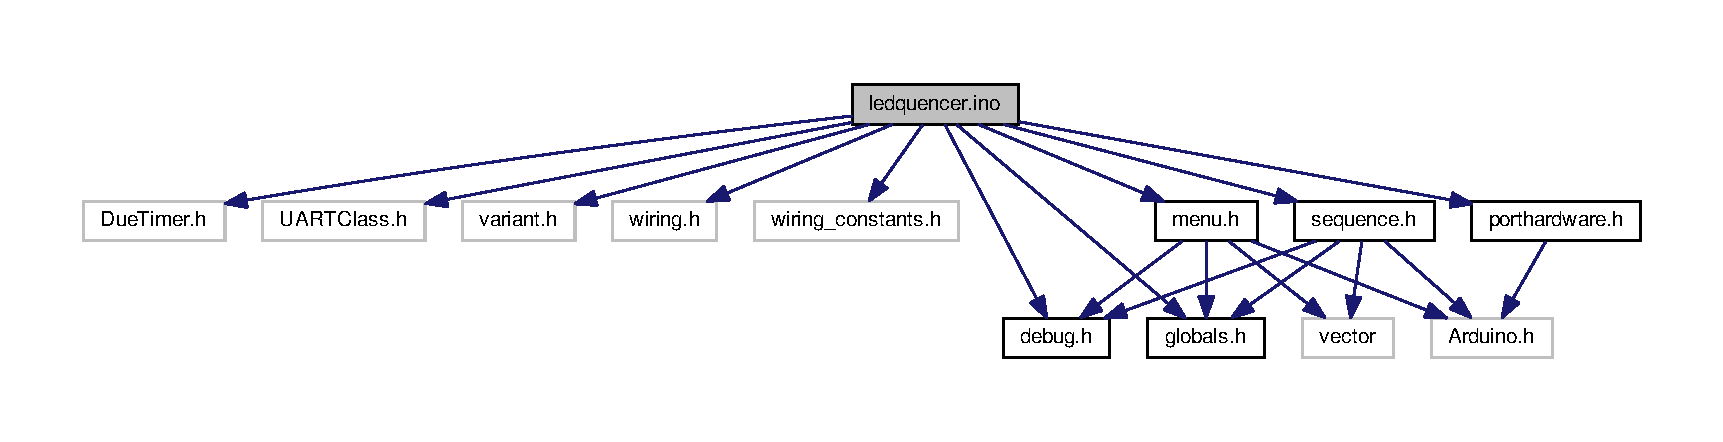
\includegraphics[width=350pt]{ledquencer_8ino__incl}
\end{center}
\end{figure}
This graph shows which files directly or indirectly include this file\-:\nopagebreak
\begin{figure}[H]
\begin{center}
\leavevmode
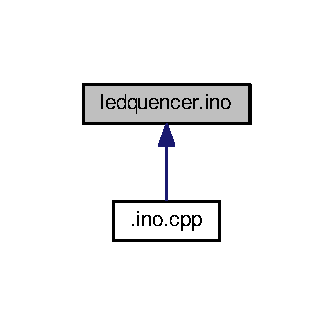
\includegraphics[width=160pt]{ledquencer_8ino__dep__incl}
\end{center}
\end{figure}
\subsection*{Functions}
\begin{DoxyCompactItemize}
\item 
void \hyperlink{ledquencer_8ino_a92c00e5adb1836741614c6492982e306}{alive1} ()
\item 
void \hyperlink{ledquencer_8ino_a859467c5035bc8e63b57dfe199caec30}{test} (int page, int buttons)
\item 
void \hyperlink{ledquencer_8ino_a4fc01d736fe50cf5b977f755b675f11d}{setup} ()
\item 
void \hyperlink{ledquencer_8ino_afe461d27b9c48d5921c00d521181f12f}{loop} ()
\item 
void \hyperlink{ledquencer_8ino_a36f33b2b623ea070c4ebccc7464ef489}{timer0\-\_\-handler} ()
\item 
void \hyperlink{ledquencer_8ino_a859aab5acbfa52240ec73ba136fb6bf3}{timer1\-\_\-handler} ()
\item 
void \hyperlink{ledquencer_8ino_a7cbb97684327369274bcf81b967c3a6b}{timer2\-\_\-handler} ()
\item 
void \hyperlink{ledquencer_8ino_a21338471d58456b6ec2c6b0070e44d67}{timer3\-\_\-handler} ()
\end{DoxyCompactItemize}
\subsection*{Variables}
\begin{DoxyCompactItemize}
\item 
int \hyperlink{ledquencer_8ino_a0f5109855ecd58cd3b97d093ac9815f2}{debugging\-\_\-enabled} = 1
\item 
long \hyperlink{ledquencer_8ino_a52bbd9d1a2fe4882a744f1e7092f5d99}{sam\-\_\-millis} = 0
\item 
volatile int \hyperlink{ledquencer_8ino_a58398a8d155ae453dfb8b9934f63484d}{posi} = 0
\item 
bool \hyperlink{ledquencer_8ino_a6009df3a7743868edbf59608b4781190}{send\-\_\-debug} = false
\item 
long \hyperlink{ledquencer_8ino_a4c14e9bc13ac36ecb3331ff5bb765816}{vorher} = 0
\item 
\hyperlink{classMenu}{Menu} \hyperlink{ledquencer_8ino_a2ad0f4be462ff63c3c72779e80988d15}{menu} = \hyperlink{classMenu}{Menu}()
\end{DoxyCompactItemize}


\subsection{Function Documentation}
\hypertarget{ledquencer_8ino_a92c00e5adb1836741614c6492982e306}{\index{ledquencer.\-ino@{ledquencer.\-ino}!alive1@{alive1}}
\index{alive1@{alive1}!ledquencer.ino@{ledquencer.\-ino}}
\subsubsection[{alive1}]{\setlength{\rightskip}{0pt plus 5cm}void alive1 (
\begin{DoxyParamCaption}
{}
\end{DoxyParamCaption}
)}}\label{ledquencer_8ino_a92c00e5adb1836741614c6492982e306}
\hypertarget{ledquencer_8ino_afe461d27b9c48d5921c00d521181f12f}{\index{ledquencer.\-ino@{ledquencer.\-ino}!loop@{loop}}
\index{loop@{loop}!ledquencer.ino@{ledquencer.\-ino}}
\subsubsection[{loop}]{\setlength{\rightskip}{0pt plus 5cm}void loop (
\begin{DoxyParamCaption}
{}
\end{DoxyParamCaption}
)}}\label{ledquencer_8ino_afe461d27b9c48d5921c00d521181f12f}
\hypertarget{ledquencer_8ino_a4fc01d736fe50cf5b977f755b675f11d}{\index{ledquencer.\-ino@{ledquencer.\-ino}!setup@{setup}}
\index{setup@{setup}!ledquencer.ino@{ledquencer.\-ino}}
\subsubsection[{setup}]{\setlength{\rightskip}{0pt plus 5cm}void setup (
\begin{DoxyParamCaption}
{}
\end{DoxyParamCaption}
)}}\label{ledquencer_8ino_a4fc01d736fe50cf5b977f755b675f11d}
\hypertarget{ledquencer_8ino_a859467c5035bc8e63b57dfe199caec30}{\index{ledquencer.\-ino@{ledquencer.\-ino}!test@{test}}
\index{test@{test}!ledquencer.ino@{ledquencer.\-ino}}
\subsubsection[{test}]{\setlength{\rightskip}{0pt plus 5cm}void test (
\begin{DoxyParamCaption}
\item[{int}]{page, }
\item[{int}]{buttons}
\end{DoxyParamCaption}
)}}\label{ledquencer_8ino_a859467c5035bc8e63b57dfe199caec30}
\hypertarget{ledquencer_8ino_a36f33b2b623ea070c4ebccc7464ef489}{\index{ledquencer.\-ino@{ledquencer.\-ino}!timer0\-\_\-handler@{timer0\-\_\-handler}}
\index{timer0\-\_\-handler@{timer0\-\_\-handler}!ledquencer.ino@{ledquencer.\-ino}}
\subsubsection[{timer0\-\_\-handler}]{\setlength{\rightskip}{0pt plus 5cm}void timer0\-\_\-handler (
\begin{DoxyParamCaption}
{}
\end{DoxyParamCaption}
)}}\label{ledquencer_8ino_a36f33b2b623ea070c4ebccc7464ef489}
\hypertarget{ledquencer_8ino_a859aab5acbfa52240ec73ba136fb6bf3}{\index{ledquencer.\-ino@{ledquencer.\-ino}!timer1\-\_\-handler@{timer1\-\_\-handler}}
\index{timer1\-\_\-handler@{timer1\-\_\-handler}!ledquencer.ino@{ledquencer.\-ino}}
\subsubsection[{timer1\-\_\-handler}]{\setlength{\rightskip}{0pt plus 5cm}void timer1\-\_\-handler (
\begin{DoxyParamCaption}
{}
\end{DoxyParamCaption}
)}}\label{ledquencer_8ino_a859aab5acbfa52240ec73ba136fb6bf3}
\hypertarget{ledquencer_8ino_a7cbb97684327369274bcf81b967c3a6b}{\index{ledquencer.\-ino@{ledquencer.\-ino}!timer2\-\_\-handler@{timer2\-\_\-handler}}
\index{timer2\-\_\-handler@{timer2\-\_\-handler}!ledquencer.ino@{ledquencer.\-ino}}
\subsubsection[{timer2\-\_\-handler}]{\setlength{\rightskip}{0pt plus 5cm}void timer2\-\_\-handler (
\begin{DoxyParamCaption}
{}
\end{DoxyParamCaption}
)}}\label{ledquencer_8ino_a7cbb97684327369274bcf81b967c3a6b}
\hypertarget{ledquencer_8ino_a21338471d58456b6ec2c6b0070e44d67}{\index{ledquencer.\-ino@{ledquencer.\-ino}!timer3\-\_\-handler@{timer3\-\_\-handler}}
\index{timer3\-\_\-handler@{timer3\-\_\-handler}!ledquencer.ino@{ledquencer.\-ino}}
\subsubsection[{timer3\-\_\-handler}]{\setlength{\rightskip}{0pt plus 5cm}void timer3\-\_\-handler (
\begin{DoxyParamCaption}
{}
\end{DoxyParamCaption}
)}}\label{ledquencer_8ino_a21338471d58456b6ec2c6b0070e44d67}


\subsection{Variable Documentation}
\hypertarget{ledquencer_8ino_a0f5109855ecd58cd3b97d093ac9815f2}{\index{ledquencer.\-ino@{ledquencer.\-ino}!debugging\-\_\-enabled@{debugging\-\_\-enabled}}
\index{debugging\-\_\-enabled@{debugging\-\_\-enabled}!ledquencer.ino@{ledquencer.\-ino}}
\subsubsection[{debugging\-\_\-enabled}]{\setlength{\rightskip}{0pt plus 5cm}int debugging\-\_\-enabled = 1}}\label{ledquencer_8ino_a0f5109855ecd58cd3b97d093ac9815f2}
\hypertarget{ledquencer_8ino_a2ad0f4be462ff63c3c72779e80988d15}{\index{ledquencer.\-ino@{ledquencer.\-ino}!menu@{menu}}
\index{menu@{menu}!ledquencer.ino@{ledquencer.\-ino}}
\subsubsection[{menu}]{\setlength{\rightskip}{0pt plus 5cm}{\bf Menu} menu = {\bf Menu}()}}\label{ledquencer_8ino_a2ad0f4be462ff63c3c72779e80988d15}
\hypertarget{ledquencer_8ino_a58398a8d155ae453dfb8b9934f63484d}{\index{ledquencer.\-ino@{ledquencer.\-ino}!posi@{posi}}
\index{posi@{posi}!ledquencer.ino@{ledquencer.\-ino}}
\subsubsection[{posi}]{\setlength{\rightskip}{0pt plus 5cm}volatile int posi = 0}}\label{ledquencer_8ino_a58398a8d155ae453dfb8b9934f63484d}
\hypertarget{ledquencer_8ino_a52bbd9d1a2fe4882a744f1e7092f5d99}{\index{ledquencer.\-ino@{ledquencer.\-ino}!sam\-\_\-millis@{sam\-\_\-millis}}
\index{sam\-\_\-millis@{sam\-\_\-millis}!ledquencer.ino@{ledquencer.\-ino}}
\subsubsection[{sam\-\_\-millis}]{\setlength{\rightskip}{0pt plus 5cm}long sam\-\_\-millis = 0}}\label{ledquencer_8ino_a52bbd9d1a2fe4882a744f1e7092f5d99}
\hypertarget{ledquencer_8ino_a6009df3a7743868edbf59608b4781190}{\index{ledquencer.\-ino@{ledquencer.\-ino}!send\-\_\-debug@{send\-\_\-debug}}
\index{send\-\_\-debug@{send\-\_\-debug}!ledquencer.ino@{ledquencer.\-ino}}
\subsubsection[{send\-\_\-debug}]{\setlength{\rightskip}{0pt plus 5cm}bool send\-\_\-debug = false}}\label{ledquencer_8ino_a6009df3a7743868edbf59608b4781190}
\hypertarget{ledquencer_8ino_a4c14e9bc13ac36ecb3331ff5bb765816}{\index{ledquencer.\-ino@{ledquencer.\-ino}!vorher@{vorher}}
\index{vorher@{vorher}!ledquencer.ino@{ledquencer.\-ino}}
\subsubsection[{vorher}]{\setlength{\rightskip}{0pt plus 5cm}long vorher = 0}}\label{ledquencer_8ino_a4c14e9bc13ac36ecb3331ff5bb765816}

\hypertarget{ledtest_8h}{\section{ledtest.\-h File Reference}
\label{ledtest_8h}\index{ledtest.\-h@{ledtest.\-h}}
}
\subsection*{Functions}
\begin{DoxyCompactItemize}
\item 
uint32\-\_\-t \hyperlink{ledtest_8h_a953424274959481c9d46b57d249b3722}{Wheel} (byte Wheel\-Pos)
\item 
void \hyperlink{ledtest_8h_aeed18d3bd1eb7b9d8626d1f282e4e634}{color\-Wipe} (uint32\-\_\-t c, uint8\-\_\-t wait)
\item 
void \hyperlink{ledtest_8h_a165da20a382814e9b9180c1aad001705}{rainbow} (uint8\-\_\-t wait)
\item 
void \hyperlink{ledtest_8h_af1139176e0556c3b4d982e85410c4a88}{rainbow\-Cycle} (uint8\-\_\-t wait)
\item 
void \hyperlink{ledtest_8h_a4a4bae8409f11ecb06e5a7a636d2831f}{theater\-Chase} (uint32\-\_\-t c, uint8\-\_\-t wait)
\item 
void \hyperlink{ledtest_8h_a5c88041adf7cb51c661fec00054b620f}{theater\-Chase\-Rainbow} (uint8\-\_\-t wait)
\end{DoxyCompactItemize}


\subsection{Function Documentation}
\hypertarget{ledtest_8h_aeed18d3bd1eb7b9d8626d1f282e4e634}{\index{ledtest.\-h@{ledtest.\-h}!color\-Wipe@{color\-Wipe}}
\index{color\-Wipe@{color\-Wipe}!ledtest.h@{ledtest.\-h}}
\subsubsection[{color\-Wipe}]{\setlength{\rightskip}{0pt plus 5cm}void color\-Wipe (
\begin{DoxyParamCaption}
\item[{uint32\-\_\-t}]{c, }
\item[{uint8\-\_\-t}]{wait}
\end{DoxyParamCaption}
)}}\label{ledtest_8h_aeed18d3bd1eb7b9d8626d1f282e4e634}
\hypertarget{ledtest_8h_a165da20a382814e9b9180c1aad001705}{\index{ledtest.\-h@{ledtest.\-h}!rainbow@{rainbow}}
\index{rainbow@{rainbow}!ledtest.h@{ledtest.\-h}}
\subsubsection[{rainbow}]{\setlength{\rightskip}{0pt plus 5cm}void rainbow (
\begin{DoxyParamCaption}
\item[{uint8\-\_\-t}]{wait}
\end{DoxyParamCaption}
)}}\label{ledtest_8h_a165da20a382814e9b9180c1aad001705}
\hypertarget{ledtest_8h_af1139176e0556c3b4d982e85410c4a88}{\index{ledtest.\-h@{ledtest.\-h}!rainbow\-Cycle@{rainbow\-Cycle}}
\index{rainbow\-Cycle@{rainbow\-Cycle}!ledtest.h@{ledtest.\-h}}
\subsubsection[{rainbow\-Cycle}]{\setlength{\rightskip}{0pt plus 5cm}void rainbow\-Cycle (
\begin{DoxyParamCaption}
\item[{uint8\-\_\-t}]{wait}
\end{DoxyParamCaption}
)}}\label{ledtest_8h_af1139176e0556c3b4d982e85410c4a88}
\hypertarget{ledtest_8h_a4a4bae8409f11ecb06e5a7a636d2831f}{\index{ledtest.\-h@{ledtest.\-h}!theater\-Chase@{theater\-Chase}}
\index{theater\-Chase@{theater\-Chase}!ledtest.h@{ledtest.\-h}}
\subsubsection[{theater\-Chase}]{\setlength{\rightskip}{0pt plus 5cm}void theater\-Chase (
\begin{DoxyParamCaption}
\item[{uint32\-\_\-t}]{c, }
\item[{uint8\-\_\-t}]{wait}
\end{DoxyParamCaption}
)}}\label{ledtest_8h_a4a4bae8409f11ecb06e5a7a636d2831f}
\hypertarget{ledtest_8h_a5c88041adf7cb51c661fec00054b620f}{\index{ledtest.\-h@{ledtest.\-h}!theater\-Chase\-Rainbow@{theater\-Chase\-Rainbow}}
\index{theater\-Chase\-Rainbow@{theater\-Chase\-Rainbow}!ledtest.h@{ledtest.\-h}}
\subsubsection[{theater\-Chase\-Rainbow}]{\setlength{\rightskip}{0pt plus 5cm}void theater\-Chase\-Rainbow (
\begin{DoxyParamCaption}
\item[{uint8\-\_\-t}]{wait}
\end{DoxyParamCaption}
)}}\label{ledtest_8h_a5c88041adf7cb51c661fec00054b620f}
\hypertarget{ledtest_8h_a953424274959481c9d46b57d249b3722}{\index{ledtest.\-h@{ledtest.\-h}!Wheel@{Wheel}}
\index{Wheel@{Wheel}!ledtest.h@{ledtest.\-h}}
\subsubsection[{Wheel}]{\setlength{\rightskip}{0pt plus 5cm}uint32\-\_\-t Wheel (
\begin{DoxyParamCaption}
\item[{byte}]{Wheel\-Pos}
\end{DoxyParamCaption}
)}}\label{ledtest_8h_a953424274959481c9d46b57d249b3722}

\hypertarget{menu_8cpp}{\section{menu.\-cpp File Reference}
\label{menu_8cpp}\index{menu.\-cpp@{menu.\-cpp}}
}
{\ttfamily \#include \char`\"{}menu.\-h\char`\"{}}\\*
Include dependency graph for menu.\-cpp\-:\nopagebreak
\begin{figure}[H]
\begin{center}
\leavevmode
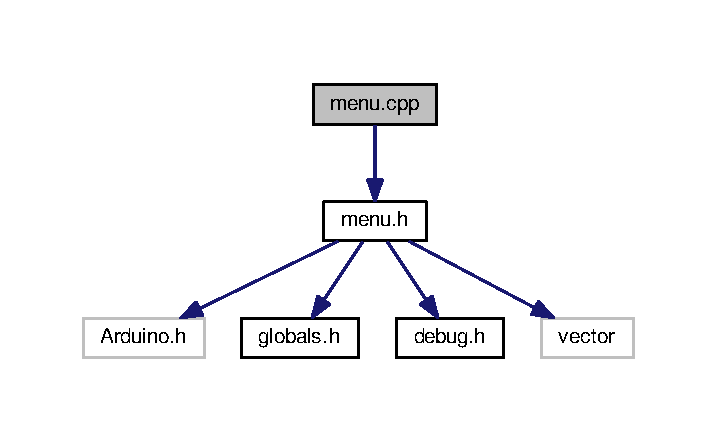
\includegraphics[width=344pt]{menu_8cpp__incl}
\end{center}
\end{figure}

\hypertarget{menu_8h}{\section{menu.\-h File Reference}
\label{menu_8h}\index{menu.\-h@{menu.\-h}}
}
{\ttfamily \#include \char`\"{}Arduino.\-h\char`\"{}}\\*
{\ttfamily \#include \char`\"{}globals.\-h\char`\"{}}\\*
{\ttfamily \#include \char`\"{}debug.\-h\char`\"{}}\\*
{\ttfamily \#include $<$vector$>$}\\*
Include dependency graph for menu.\-h\-:\nopagebreak
\begin{figure}[H]
\begin{center}
\leavevmode
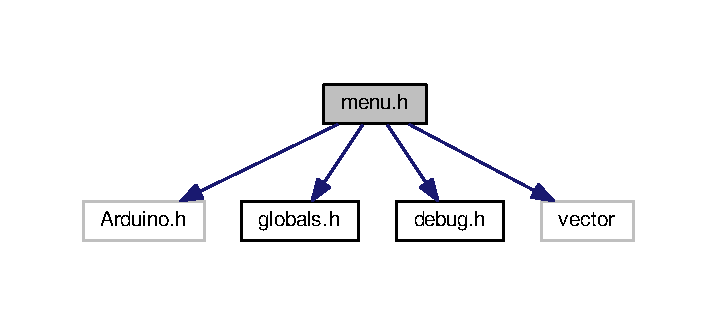
\includegraphics[width=344pt]{menu_8h__incl}
\end{center}
\end{figure}
This graph shows which files directly or indirectly include this file\-:\nopagebreak
\begin{figure}[H]
\begin{center}
\leavevmode
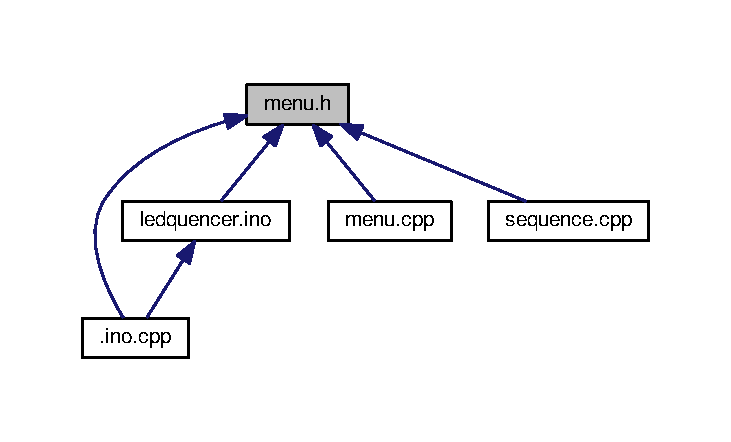
\includegraphics[width=350pt]{menu_8h__dep__incl}
\end{center}
\end{figure}
\subsection*{Classes}
\begin{DoxyCompactItemize}
\item 
class \hyperlink{classMenu}{Menu}
\begin{DoxyCompactList}\small\item\em menu class for menu handling. \end{DoxyCompactList}\end{DoxyCompactItemize}
\subsection*{Namespaces}
\begin{DoxyCompactItemize}
\item 
\hyperlink{namespaceMenuEnums}{Menu\-Enums}
\begin{DoxyCompactList}\small\item\em menu enumerations. \end{DoxyCompactList}\end{DoxyCompactItemize}
\subsection*{Enumerations}
\begin{DoxyCompactItemize}
\item 
enum \hyperlink{namespaceMenuEnums_a8a0112033fd82b21fb91024f2da815db}{Menu\-Enums\-::e\-\_\-menu\-\_\-buttons} \{ \\*
\hyperlink{namespaceMenuEnums_a8a0112033fd82b21fb91024f2da815dba35174bcb834b5288e617b5e403916282}{Menu\-Enums\-::\-Main} = 0, 
\hyperlink{namespaceMenuEnums_a8a0112033fd82b21fb91024f2da815dbac342bed09bcc9a5d2e4c80c6cbac4e42}{Menu\-Enums\-::\-Sequence} = 1, 
\hyperlink{namespaceMenuEnums_a8a0112033fd82b21fb91024f2da815dba3775e44f7da30c57fe300475a573e024}{Menu\-Enums\-::\-Pattern} = 2, 
\hyperlink{namespaceMenuEnums_a8a0112033fd82b21fb91024f2da815dbafc27e347494357604e497db2c2a07be0}{Menu\-Enums\-::\-Out} = 4, 
\\*
\hyperlink{namespaceMenuEnums_a8a0112033fd82b21fb91024f2da815dbad31732cb8f9cbf4c6d27adcc749bc636}{Menu\-Enums\-::\-Cycle} = 8, 
\hyperlink{namespaceMenuEnums_a8a0112033fd82b21fb91024f2da815dbaf1ead4564553031959e56857c8f29b57}{Menu\-Enums\-::\-Solo} = 16, 
\hyperlink{namespaceMenuEnums_a8a0112033fd82b21fb91024f2da815dba14c45f0470352eebdf23571c855bb77d}{Menu\-Enums\-::\-Shift} = 32, 
\hyperlink{namespaceMenuEnums_a8a0112033fd82b21fb91024f2da815dba9bb0e4755281d36cb67e663da534171b}{Menu\-Enums\-::\-F\-N} = 64, 
\\*
\hyperlink{namespaceMenuEnums_a8a0112033fd82b21fb91024f2da815dba91e3e422ba63a9de93a637f0dd7ffbf5}{Menu\-Enums\-::\-Start} = 128
 \}
\begin{DoxyCompactList}\small\item\em functionbuttons enum. \end{DoxyCompactList}\end{DoxyCompactItemize}

\hypertarget{porthardware_8h}{\section{porthardware.\-h File Reference}
\label{porthardware_8h}\index{porthardware.\-h@{porthardware.\-h}}
}
{\ttfamily \#include $<$Arduino.\-h$>$}\\*
Include dependency graph for porthardware.\-h\-:\nopagebreak
\begin{figure}[H]
\begin{center}
\leavevmode
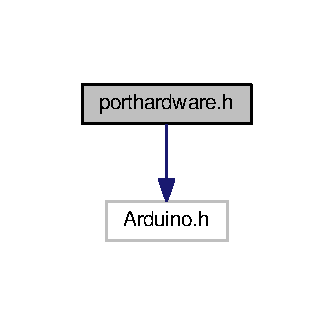
\includegraphics[width=160pt]{porthardware_8h__incl}
\end{center}
\end{figure}
This graph shows which files directly or indirectly include this file\-:\nopagebreak
\begin{figure}[H]
\begin{center}
\leavevmode
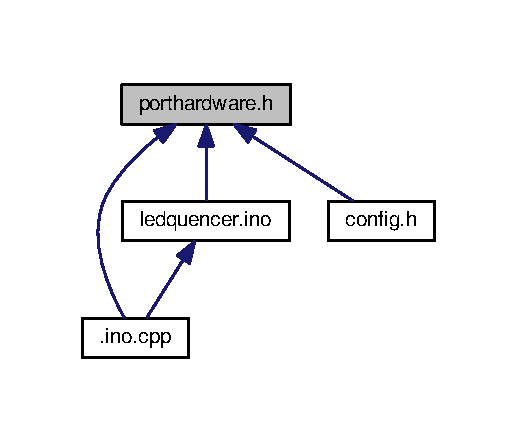
\includegraphics[width=248pt]{porthardware_8h__dep__incl}
\end{center}
\end{figure}
\subsection*{Functions}
\begin{DoxyCompactItemize}
\item 
bool \hyperlink{porthardware_8h_a7bdc13ef4eafc2bba6ca7b18e2768bdf}{get\-\_\-bit} (int val, int pos)
\item 
void \hyperlink{porthardware_8h_a9be587afe4abd5e378d7e1c2409f95fd}{readin\-S\-B} ()
\item 
void \hyperlink{porthardware_8h_adbb172da11cfebdda095fd76dd83c11f}{readin\-F\-B} ()
\item 
void \hyperlink{porthardware_8h_adf3d0f6e1a9dd64fb3ec03ec0e662bfe}{read\-Buttons} ()
\item 
void \hyperlink{porthardware_8h_acbac040cb9301bc84a906f3b5a069338}{update\-\_\-mux} (int index)
\item 
void \hyperlink{porthardware_8h_a1d1d064b66cef13f4b81725e35a5a442}{muxoutirq} (int i)
\item 
void \hyperlink{porthardware_8h_ac3536dbe68781b0f68515675320419db}{update\-\_\-trg} ()
\item 
void \hyperlink{porthardware_8h_a7b55b33f80d664f78718fdb04b0b9f7c}{set\-Debounce} ()
\item 
void \hyperlink{porthardware_8h_ad8d6aca3d85765fb35287d8f9bad21d1}{portsetup} ()
\end{DoxyCompactItemize}
\subsection*{Variables}
\begin{DoxyCompactItemize}
\item 
bool \hyperlink{porthardware_8h_ab94e3899a08bc1399d9c8121b3df7bda}{mux1} \mbox{[}16\mbox{]}
\item 
bool \hyperlink{porthardware_8h_a8963f0416774ec8e591442f23b3a7f13}{mux2} \mbox{[}16\mbox{]}
\item 
bool \hyperlink{porthardware_8h_ae6469ec5fc1a181cbdab4ebb4da532de}{mux3} \mbox{[}16\mbox{]}
\end{DoxyCompactItemize}


\subsection{Function Documentation}
\hypertarget{porthardware_8h_a7bdc13ef4eafc2bba6ca7b18e2768bdf}{\index{porthardware.\-h@{porthardware.\-h}!get\-\_\-bit@{get\-\_\-bit}}
\index{get\-\_\-bit@{get\-\_\-bit}!porthardware.h@{porthardware.\-h}}
\subsubsection[{get\-\_\-bit}]{\setlength{\rightskip}{0pt plus 5cm}bool get\-\_\-bit (
\begin{DoxyParamCaption}
\item[{int}]{val, }
\item[{int}]{pos}
\end{DoxyParamCaption}
)}}\label{porthardware_8h_a7bdc13ef4eafc2bba6ca7b18e2768bdf}
\hypertarget{porthardware_8h_a1d1d064b66cef13f4b81725e35a5a442}{\index{porthardware.\-h@{porthardware.\-h}!muxoutirq@{muxoutirq}}
\index{muxoutirq@{muxoutirq}!porthardware.h@{porthardware.\-h}}
\subsubsection[{muxoutirq}]{\setlength{\rightskip}{0pt plus 5cm}void muxoutirq (
\begin{DoxyParamCaption}
\item[{int}]{i}
\end{DoxyParamCaption}
)}}\label{porthardware_8h_a1d1d064b66cef13f4b81725e35a5a442}
\hypertarget{porthardware_8h_ad8d6aca3d85765fb35287d8f9bad21d1}{\index{porthardware.\-h@{porthardware.\-h}!portsetup@{portsetup}}
\index{portsetup@{portsetup}!porthardware.h@{porthardware.\-h}}
\subsubsection[{portsetup}]{\setlength{\rightskip}{0pt plus 5cm}void portsetup (
\begin{DoxyParamCaption}
{}
\end{DoxyParamCaption}
)}}\label{porthardware_8h_ad8d6aca3d85765fb35287d8f9bad21d1}
\hypertarget{porthardware_8h_adf3d0f6e1a9dd64fb3ec03ec0e662bfe}{\index{porthardware.\-h@{porthardware.\-h}!read\-Buttons@{read\-Buttons}}
\index{read\-Buttons@{read\-Buttons}!porthardware.h@{porthardware.\-h}}
\subsubsection[{read\-Buttons}]{\setlength{\rightskip}{0pt plus 5cm}void read\-Buttons (
\begin{DoxyParamCaption}
{}
\end{DoxyParamCaption}
)}}\label{porthardware_8h_adf3d0f6e1a9dd64fb3ec03ec0e662bfe}
\hypertarget{porthardware_8h_adbb172da11cfebdda095fd76dd83c11f}{\index{porthardware.\-h@{porthardware.\-h}!readin\-F\-B@{readin\-F\-B}}
\index{readin\-F\-B@{readin\-F\-B}!porthardware.h@{porthardware.\-h}}
\subsubsection[{readin\-F\-B}]{\setlength{\rightskip}{0pt plus 5cm}void readin\-F\-B (
\begin{DoxyParamCaption}
{}
\end{DoxyParamCaption}
)}}\label{porthardware_8h_adbb172da11cfebdda095fd76dd83c11f}
\hypertarget{porthardware_8h_a9be587afe4abd5e378d7e1c2409f95fd}{\index{porthardware.\-h@{porthardware.\-h}!readin\-S\-B@{readin\-S\-B}}
\index{readin\-S\-B@{readin\-S\-B}!porthardware.h@{porthardware.\-h}}
\subsubsection[{readin\-S\-B}]{\setlength{\rightskip}{0pt plus 5cm}void readin\-S\-B (
\begin{DoxyParamCaption}
{}
\end{DoxyParamCaption}
)}}\label{porthardware_8h_a9be587afe4abd5e378d7e1c2409f95fd}
\hypertarget{porthardware_8h_a7b55b33f80d664f78718fdb04b0b9f7c}{\index{porthardware.\-h@{porthardware.\-h}!set\-Debounce@{set\-Debounce}}
\index{set\-Debounce@{set\-Debounce}!porthardware.h@{porthardware.\-h}}
\subsubsection[{set\-Debounce}]{\setlength{\rightskip}{0pt plus 5cm}void set\-Debounce (
\begin{DoxyParamCaption}
{}
\end{DoxyParamCaption}
)}}\label{porthardware_8h_a7b55b33f80d664f78718fdb04b0b9f7c}
\hypertarget{porthardware_8h_acbac040cb9301bc84a906f3b5a069338}{\index{porthardware.\-h@{porthardware.\-h}!update\-\_\-mux@{update\-\_\-mux}}
\index{update\-\_\-mux@{update\-\_\-mux}!porthardware.h@{porthardware.\-h}}
\subsubsection[{update\-\_\-mux}]{\setlength{\rightskip}{0pt plus 5cm}void update\-\_\-mux (
\begin{DoxyParamCaption}
\item[{int}]{index}
\end{DoxyParamCaption}
)}}\label{porthardware_8h_acbac040cb9301bc84a906f3b5a069338}
\hypertarget{porthardware_8h_ac3536dbe68781b0f68515675320419db}{\index{porthardware.\-h@{porthardware.\-h}!update\-\_\-trg@{update\-\_\-trg}}
\index{update\-\_\-trg@{update\-\_\-trg}!porthardware.h@{porthardware.\-h}}
\subsubsection[{update\-\_\-trg}]{\setlength{\rightskip}{0pt plus 5cm}void update\-\_\-trg (
\begin{DoxyParamCaption}
{}
\end{DoxyParamCaption}
)}}\label{porthardware_8h_ac3536dbe68781b0f68515675320419db}


\subsection{Variable Documentation}
\hypertarget{porthardware_8h_ab94e3899a08bc1399d9c8121b3df7bda}{\index{porthardware.\-h@{porthardware.\-h}!mux1@{mux1}}
\index{mux1@{mux1}!porthardware.h@{porthardware.\-h}}
\subsubsection[{mux1}]{\setlength{\rightskip}{0pt plus 5cm}bool mux1\mbox{[}16\mbox{]}}}\label{porthardware_8h_ab94e3899a08bc1399d9c8121b3df7bda}
\hypertarget{porthardware_8h_a8963f0416774ec8e591442f23b3a7f13}{\index{porthardware.\-h@{porthardware.\-h}!mux2@{mux2}}
\index{mux2@{mux2}!porthardware.h@{porthardware.\-h}}
\subsubsection[{mux2}]{\setlength{\rightskip}{0pt plus 5cm}bool mux2\mbox{[}16\mbox{]}}}\label{porthardware_8h_a8963f0416774ec8e591442f23b3a7f13}
\hypertarget{porthardware_8h_ae6469ec5fc1a181cbdab4ebb4da532de}{\index{porthardware.\-h@{porthardware.\-h}!mux3@{mux3}}
\index{mux3@{mux3}!porthardware.h@{porthardware.\-h}}
\subsubsection[{mux3}]{\setlength{\rightskip}{0pt plus 5cm}bool mux3\mbox{[}16\mbox{]}}}\label{porthardware_8h_ae6469ec5fc1a181cbdab4ebb4da532de}

\hypertarget{sequence_8cpp}{\section{sequence.\-cpp File Reference}
\label{sequence_8cpp}\index{sequence.\-cpp@{sequence.\-cpp}}
}
{\ttfamily \#include \char`\"{}Arduino.\-h\char`\"{}}\\*
{\ttfamily \#include \char`\"{}sequence.\-h\char`\"{}}\\*
{\ttfamily \#include \char`\"{}menu.\-h\char`\"{}}\\*
Include dependency graph for sequence.\-cpp\-:\nopagebreak
\begin{figure}[H]
\begin{center}
\leavevmode
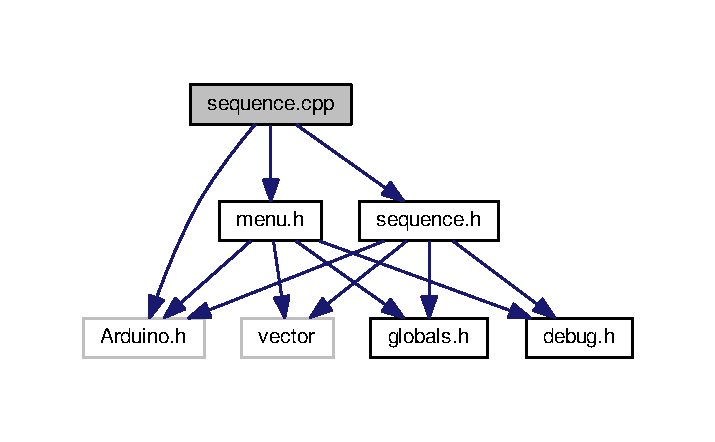
\includegraphics[width=343pt]{sequence_8cpp__incl}
\end{center}
\end{figure}
\subsection*{Functions}
\begin{DoxyCompactItemize}
\item 
void \hyperlink{sequence_8cpp_a134a45f4b0e8d503a31efd86fee48292}{Callback} (\hyperlink{classSequence}{Sequence} $\ast$instance, int x)
\end{DoxyCompactItemize}


\subsection{Function Documentation}
\hypertarget{sequence_8cpp_a134a45f4b0e8d503a31efd86fee48292}{\index{sequence.\-cpp@{sequence.\-cpp}!Callback@{Callback}}
\index{Callback@{Callback}!sequence.cpp@{sequence.\-cpp}}
\subsubsection[{Callback}]{\setlength{\rightskip}{0pt plus 5cm}void Callback (
\begin{DoxyParamCaption}
\item[{{\bf Sequence} $\ast$}]{instance, }
\item[{int}]{x}
\end{DoxyParamCaption}
)}}\label{sequence_8cpp_a134a45f4b0e8d503a31efd86fee48292}

\hypertarget{sequence_8h}{\section{sequence.\-h File Reference}
\label{sequence_8h}\index{sequence.\-h@{sequence.\-h}}
}
{\ttfamily \#include $<$vector$>$}\\*
{\ttfamily \#include \char`\"{}Arduino.\-h\char`\"{}}\\*
{\ttfamily \#include \char`\"{}globals.\-h\char`\"{}}\\*
{\ttfamily \#include \char`\"{}debug.\-h\char`\"{}}\\*
Include dependency graph for sequence.\-h\-:\nopagebreak
\begin{figure}[H]
\begin{center}
\leavevmode
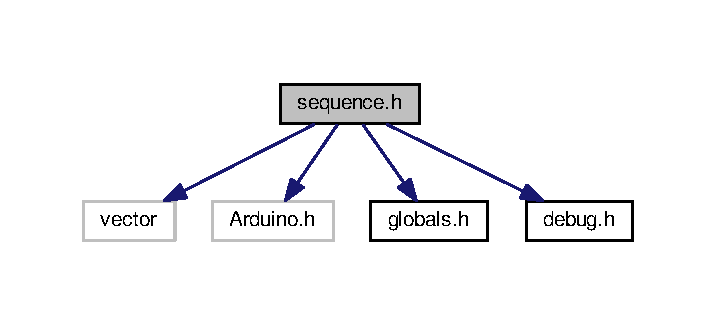
\includegraphics[width=343pt]{sequence_8h__incl}
\end{center}
\end{figure}
This graph shows which files directly or indirectly include this file\-:
\nopagebreak
\begin{figure}[H]
\begin{center}
\leavevmode
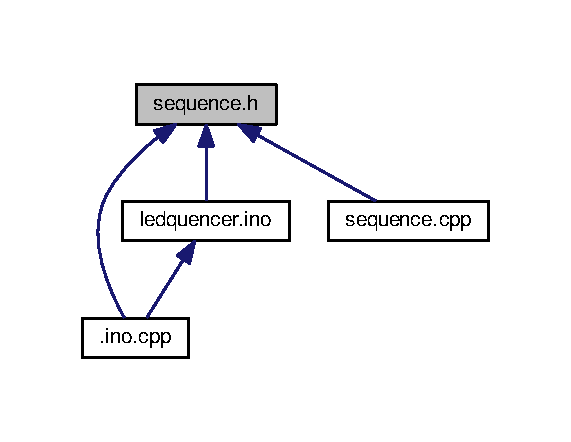
\includegraphics[width=274pt]{sequence_8h__dep__incl}
\end{center}
\end{figure}
\subsection*{Classes}
\begin{DoxyCompactItemize}
\item 
struct \hyperlink{structSequenceEnum_1_1StepData}{Sequence\-Enum\-::\-Step\-Data}
\begin{DoxyCompactList}\small\item\em Basic struct of one step -\/ data. used on all step data operations. \end{DoxyCompactList}\item 
struct \hyperlink{structSequenceEnum_1_1SequenceMeta}{Sequence\-Enum\-::\-Sequence\-Meta}
\begin{DoxyCompactList}\small\item\em some ssquence metadata for internal handling \end{DoxyCompactList}\item 
class \hyperlink{classSequence}{Sequence}
\begin{DoxyCompactList}\small\item\em \hyperlink{classSequence}{Sequence} class. \end{DoxyCompactList}\end{DoxyCompactItemize}
\subsection*{Namespaces}
\begin{DoxyCompactItemize}
\item 
\hyperlink{namespaceSequenceEnum}{Sequence\-Enum}
\begin{DoxyCompactList}\small\item\em This is the sequence data namespace.\par
 it defines sequence related enumerations used across the programm. \end{DoxyCompactList}\end{DoxyCompactItemize}
\subsection*{Enumerations}
\begin{DoxyCompactItemize}
\item 
enum \hyperlink{namespaceSequenceEnum_ac7ea8369c971b81acfe5a1d63a10ebe3}{Sequence\-Enum\-::e\-\_\-run\-States} \{ \\*
\hyperlink{namespaceSequenceEnum_ac7ea8369c971b81acfe5a1d63a10ebe3aba765510708832ec607eb5916f07fd35}{Sequence\-Enum\-::\-Run}, 
\hyperlink{namespaceSequenceEnum_ac7ea8369c971b81acfe5a1d63a10ebe3aa9ca5b61780cadeed0d5963095fe5db5}{Sequence\-Enum\-::\-Start}, 
\hyperlink{namespaceSequenceEnum_ac7ea8369c971b81acfe5a1d63a10ebe3aa277d3642c16a5f3597cf49ff021abff}{Sequence\-Enum\-::\-Restart}, 
\hyperlink{namespaceSequenceEnum_ac7ea8369c971b81acfe5a1d63a10ebe3a9a4e6acbff3104211a16c87ebe5b7a58}{Sequence\-Enum\-::\-Stop}, 
\\*
\hyperlink{namespaceSequenceEnum_ac7ea8369c971b81acfe5a1d63a10ebe3ac384cac9192fd9e1def2767b7e7620d4}{Sequence\-Enum\-::\-Pause}, 
\hyperlink{namespaceSequenceEnum_ac7ea8369c971b81acfe5a1d63a10ebe3aac7d742b92696400bf6ebb628a934bf4}{Sequence\-Enum\-::\-Reset}
 \}
\item 
enum \hyperlink{namespaceSequenceEnum_a2241436a1b94492d5f8df2f01a858857}{Sequence\-Enum\-::e\-\_\-run\-Mode} \{ \\*
\hyperlink{namespaceSequenceEnum_a2241436a1b94492d5f8df2f01a858857a680c3bf17dd73fb62741d87a04f98003}{Sequence\-Enum\-::\-Forward}, 
\hyperlink{namespaceSequenceEnum_a2241436a1b94492d5f8df2f01a858857af792bbd5445c7cae1c3132f15be51bb3}{Sequence\-Enum\-::\-Backward}, 
\hyperlink{namespaceSequenceEnum_a2241436a1b94492d5f8df2f01a858857a6e24874edb554db76221d23abba33793}{Sequence\-Enum\-::\-Pendulum}, 
\hyperlink{namespaceSequenceEnum_a2241436a1b94492d5f8df2f01a858857aa496073028085d359012beb35fbfbd5a}{Sequence\-Enum\-::\-Random}, 
\\*
\hyperlink{namespaceSequenceEnum_a2241436a1b94492d5f8df2f01a858857a0d9f27ad3750aba023a973ead8dbecb8}{Sequence\-Enum\-::\-Brownian}
 \}
\end{DoxyCompactItemize}
\subsection*{Variables}
\begin{DoxyCompactItemize}
\item 
int \hyperlink{sequence_8h_a00e330408ecfcef55bd1099010754017}{patlen}
\end{DoxyCompactItemize}


\subsection{Variable Documentation}
\hypertarget{sequence_8h_a00e330408ecfcef55bd1099010754017}{\index{sequence.\-h@{sequence.\-h}!patlen@{patlen}}
\index{patlen@{patlen}!sequence.h@{sequence.\-h}}
\subsubsection[{patlen}]{\setlength{\rightskip}{0pt plus 5cm}int patlen}}\label{sequence_8h_a00e330408ecfcef55bd1099010754017}

%--- End generated contents ---

% Index
\newpage
\phantomsection
\addcontentsline{toc}{chapter}{Index}
\printindex

\end{document}
